% Options for packages loaded elsewhere
\PassOptionsToPackage{unicode}{hyperref}
\PassOptionsToPackage{hyphens}{url}
\PassOptionsToPackage{dvipsnames,svgnames,x11names}{xcolor}
%
\documentclass[
  letterpaper,
  DIV=11,
  numbers=noendperiod]{scrartcl}

\usepackage{amsmath,amssymb}
\usepackage{iftex}
\ifPDFTeX
  \usepackage[T1]{fontenc}
  \usepackage[utf8]{inputenc}
  \usepackage{textcomp} % provide euro and other symbols
\else % if luatex or xetex
  \usepackage{unicode-math}
  \defaultfontfeatures{Scale=MatchLowercase}
  \defaultfontfeatures[\rmfamily]{Ligatures=TeX,Scale=1}
\fi
\usepackage{lmodern}
\ifPDFTeX\else  
    % xetex/luatex font selection
\fi
% Use upquote if available, for straight quotes in verbatim environments
\IfFileExists{upquote.sty}{\usepackage{upquote}}{}
\IfFileExists{microtype.sty}{% use microtype if available
  \usepackage[]{microtype}
  \UseMicrotypeSet[protrusion]{basicmath} % disable protrusion for tt fonts
}{}
\makeatletter
\@ifundefined{KOMAClassName}{% if non-KOMA class
  \IfFileExists{parskip.sty}{%
    \usepackage{parskip}
  }{% else
    \setlength{\parindent}{0pt}
    \setlength{\parskip}{6pt plus 2pt minus 1pt}}
}{% if KOMA class
  \KOMAoptions{parskip=half}}
\makeatother
\usepackage{xcolor}
\setlength{\emergencystretch}{3em} % prevent overfull lines
\setcounter{secnumdepth}{5}
% Make \paragraph and \subparagraph free-standing
\makeatletter
\ifx\paragraph\undefined\else
  \let\oldparagraph\paragraph
  \renewcommand{\paragraph}{
    \@ifstar
      \xxxParagraphStar
      \xxxParagraphNoStar
  }
  \newcommand{\xxxParagraphStar}[1]{\oldparagraph*{#1}\mbox{}}
  \newcommand{\xxxParagraphNoStar}[1]{\oldparagraph{#1}\mbox{}}
\fi
\ifx\subparagraph\undefined\else
  \let\oldsubparagraph\subparagraph
  \renewcommand{\subparagraph}{
    \@ifstar
      \xxxSubParagraphStar
      \xxxSubParagraphNoStar
  }
  \newcommand{\xxxSubParagraphStar}[1]{\oldsubparagraph*{#1}\mbox{}}
  \newcommand{\xxxSubParagraphNoStar}[1]{\oldsubparagraph{#1}\mbox{}}
\fi
\makeatother

\usepackage{color}
\usepackage{fancyvrb}
\newcommand{\VerbBar}{|}
\newcommand{\VERB}{\Verb[commandchars=\\\{\}]}
\DefineVerbatimEnvironment{Highlighting}{Verbatim}{commandchars=\\\{\}}
% Add ',fontsize=\small' for more characters per line
\usepackage{framed}
\definecolor{shadecolor}{RGB}{241,243,245}
\newenvironment{Shaded}{\begin{snugshade}}{\end{snugshade}}
\newcommand{\AlertTok}[1]{\textcolor[rgb]{0.68,0.00,0.00}{#1}}
\newcommand{\AnnotationTok}[1]{\textcolor[rgb]{0.37,0.37,0.37}{#1}}
\newcommand{\AttributeTok}[1]{\textcolor[rgb]{0.40,0.45,0.13}{#1}}
\newcommand{\BaseNTok}[1]{\textcolor[rgb]{0.68,0.00,0.00}{#1}}
\newcommand{\BuiltInTok}[1]{\textcolor[rgb]{0.00,0.23,0.31}{#1}}
\newcommand{\CharTok}[1]{\textcolor[rgb]{0.13,0.47,0.30}{#1}}
\newcommand{\CommentTok}[1]{\textcolor[rgb]{0.37,0.37,0.37}{#1}}
\newcommand{\CommentVarTok}[1]{\textcolor[rgb]{0.37,0.37,0.37}{\textit{#1}}}
\newcommand{\ConstantTok}[1]{\textcolor[rgb]{0.56,0.35,0.01}{#1}}
\newcommand{\ControlFlowTok}[1]{\textcolor[rgb]{0.00,0.23,0.31}{\textbf{#1}}}
\newcommand{\DataTypeTok}[1]{\textcolor[rgb]{0.68,0.00,0.00}{#1}}
\newcommand{\DecValTok}[1]{\textcolor[rgb]{0.68,0.00,0.00}{#1}}
\newcommand{\DocumentationTok}[1]{\textcolor[rgb]{0.37,0.37,0.37}{\textit{#1}}}
\newcommand{\ErrorTok}[1]{\textcolor[rgb]{0.68,0.00,0.00}{#1}}
\newcommand{\ExtensionTok}[1]{\textcolor[rgb]{0.00,0.23,0.31}{#1}}
\newcommand{\FloatTok}[1]{\textcolor[rgb]{0.68,0.00,0.00}{#1}}
\newcommand{\FunctionTok}[1]{\textcolor[rgb]{0.28,0.35,0.67}{#1}}
\newcommand{\ImportTok}[1]{\textcolor[rgb]{0.00,0.46,0.62}{#1}}
\newcommand{\InformationTok}[1]{\textcolor[rgb]{0.37,0.37,0.37}{#1}}
\newcommand{\KeywordTok}[1]{\textcolor[rgb]{0.00,0.23,0.31}{\textbf{#1}}}
\newcommand{\NormalTok}[1]{\textcolor[rgb]{0.00,0.23,0.31}{#1}}
\newcommand{\OperatorTok}[1]{\textcolor[rgb]{0.37,0.37,0.37}{#1}}
\newcommand{\OtherTok}[1]{\textcolor[rgb]{0.00,0.23,0.31}{#1}}
\newcommand{\PreprocessorTok}[1]{\textcolor[rgb]{0.68,0.00,0.00}{#1}}
\newcommand{\RegionMarkerTok}[1]{\textcolor[rgb]{0.00,0.23,0.31}{#1}}
\newcommand{\SpecialCharTok}[1]{\textcolor[rgb]{0.37,0.37,0.37}{#1}}
\newcommand{\SpecialStringTok}[1]{\textcolor[rgb]{0.13,0.47,0.30}{#1}}
\newcommand{\StringTok}[1]{\textcolor[rgb]{0.13,0.47,0.30}{#1}}
\newcommand{\VariableTok}[1]{\textcolor[rgb]{0.07,0.07,0.07}{#1}}
\newcommand{\VerbatimStringTok}[1]{\textcolor[rgb]{0.13,0.47,0.30}{#1}}
\newcommand{\WarningTok}[1]{\textcolor[rgb]{0.37,0.37,0.37}{\textit{#1}}}

\providecommand{\tightlist}{%
  \setlength{\itemsep}{0pt}\setlength{\parskip}{0pt}}\usepackage{longtable,booktabs,array}
\usepackage{calc} % for calculating minipage widths
% Correct order of tables after \paragraph or \subparagraph
\usepackage{etoolbox}
\makeatletter
\patchcmd\longtable{\par}{\if@noskipsec\mbox{}\fi\par}{}{}
\makeatother
% Allow footnotes in longtable head/foot
\IfFileExists{footnotehyper.sty}{\usepackage{footnotehyper}}{\usepackage{footnote}}
\makesavenoteenv{longtable}
\usepackage{graphicx}
\makeatletter
\newsavebox\pandoc@box
\newcommand*\pandocbounded[1]{% scales image to fit in text height/width
  \sbox\pandoc@box{#1}%
  \Gscale@div\@tempa{\textheight}{\dimexpr\ht\pandoc@box+\dp\pandoc@box\relax}%
  \Gscale@div\@tempb{\linewidth}{\wd\pandoc@box}%
  \ifdim\@tempb\p@<\@tempa\p@\let\@tempa\@tempb\fi% select the smaller of both
  \ifdim\@tempa\p@<\p@\scalebox{\@tempa}{\usebox\pandoc@box}%
  \else\usebox{\pandoc@box}%
  \fi%
}
% Set default figure placement to htbp
\def\fps@figure{htbp}
\makeatother

% load packages
\usepackage{geometry}
\usepackage{xcolor}
\usepackage{eso-pic}
\usepackage{fancyhdr}
\usepackage{sectsty}
\usepackage{fontspec}
\usepackage{titlesec}

%% Set page size with a wider right margin
\geometry{a4paper, total={170mm,257mm}, left=20mm, top=20mm, bottom=20mm, right=50mm}

%% Let's define some colours
\definecolor{light}{HTML}{E6E6FA}
\definecolor{highlight}{HTML}{800080}
\definecolor{dark}{HTML}{330033}

%% Let's add the border on the right hand side 
\AddToShipoutPicture{% 
    \AtPageLowerLeft{% 
        \put(\LenToUnit{\dimexpr\paperwidth-3cm},0){% 
            \color{light}\rule{3cm}{\LenToUnit\paperheight}%
          }%
     }%
     % logo
    \AtPageLowerLeft{% start the bar at the bottom right of the page
        \put(\LenToUnit{\dimexpr\paperwidth-2.25cm},27.2cm){% move it to the top right
            \color{light}
\includegraphics[width=1.5cm]{_extensions/nrennie/PrettyPDF/logo.png}
          }%
     }%
}

%% Style the page number
\fancypagestyle{mystyle}{
  \fancyhf{}
  \renewcommand\headrulewidth{0pt}
  \fancyfoot[R]{\thepage}
  \fancyfootoffset{3.5cm}
}
\setlength{\footskip}{20pt}

%% style the chapter/section fonts
\chapterfont{\color{dark}\fontsize{20}{16.8}\selectfont}
\sectionfont{\color{dark}\fontsize{20}{16.8}\selectfont}
\subsectionfont{\color{dark}\fontsize{14}{16.8}\selectfont}
\titleformat{\subsection}
  {\sffamily\Large\bfseries}{\thesection}{1em}{}[{\titlerule[0.8pt]}]
  
% left align title
\makeatletter
\renewcommand{\maketitle}{\bgroup\setlength{\parindent}{0pt}
\begin{flushleft}
  {\sffamily\huge\textbf{\MakeUppercase{\@title}}} \vspace{0.3cm} \newline
  {\Large {\@subtitle}} \newline
  \@author
\end{flushleft}\egroup
}
\makeatother

%% Use some custom fonts
\setsansfont{Ubuntu}[
    Path=_extensions/nrennie/PrettyPDF/Ubuntu/,
    Scale=0.9,
    Extension = .ttf,
    UprightFont=*-Regular,
    BoldFont=*-Bold,
    ItalicFont=*-Italic,
    ]

\setmainfont{Ubuntu}[
    Path=_extensions/nrennie/PrettyPDF/Ubuntu/,
    Scale=0.9,
    Extension = .ttf,
    UprightFont=*-Regular,
    BoldFont=*-Bold,
    ItalicFont=*-Italic,
    ]
\usepackage{booktabs}
\usepackage{caption}
\usepackage{longtable}
\usepackage{colortbl}
\usepackage{array}
\usepackage{anyfontsize}
\usepackage{multirow}
\KOMAoption{captions}{tableheading}
\makeatletter
\@ifpackageloaded{tcolorbox}{}{\usepackage[skins,breakable]{tcolorbox}}
\@ifpackageloaded{fontawesome5}{}{\usepackage{fontawesome5}}
\definecolor{quarto-callout-color}{HTML}{909090}
\definecolor{quarto-callout-note-color}{HTML}{0758E5}
\definecolor{quarto-callout-important-color}{HTML}{CC1914}
\definecolor{quarto-callout-warning-color}{HTML}{EB9113}
\definecolor{quarto-callout-tip-color}{HTML}{00A047}
\definecolor{quarto-callout-caution-color}{HTML}{FC5300}
\definecolor{quarto-callout-color-frame}{HTML}{acacac}
\definecolor{quarto-callout-note-color-frame}{HTML}{4582ec}
\definecolor{quarto-callout-important-color-frame}{HTML}{d9534f}
\definecolor{quarto-callout-warning-color-frame}{HTML}{f0ad4e}
\definecolor{quarto-callout-tip-color-frame}{HTML}{02b875}
\definecolor{quarto-callout-caution-color-frame}{HTML}{fd7e14}
\makeatother
\makeatletter
\@ifpackageloaded{caption}{}{\usepackage{caption}}
\AtBeginDocument{%
\ifdefined\contentsname
  \renewcommand*\contentsname{Table of contents}
\else
  \newcommand\contentsname{Table of contents}
\fi
\ifdefined\listfigurename
  \renewcommand*\listfigurename{List of Figures}
\else
  \newcommand\listfigurename{List of Figures}
\fi
\ifdefined\listtablename
  \renewcommand*\listtablename{List of Tables}
\else
  \newcommand\listtablename{List of Tables}
\fi
\ifdefined\figurename
  \renewcommand*\figurename{Figure}
\else
  \newcommand\figurename{Figure}
\fi
\ifdefined\tablename
  \renewcommand*\tablename{Table}
\else
  \newcommand\tablename{Table}
\fi
}
\@ifpackageloaded{float}{}{\usepackage{float}}
\floatstyle{ruled}
\@ifundefined{c@chapter}{\newfloat{codelisting}{h}{lop}}{\newfloat{codelisting}{h}{lop}[chapter]}
\floatname{codelisting}{Listing}
\newcommand*\listoflistings{\listof{codelisting}{List of Listings}}
\makeatother
\makeatletter
\makeatother
\makeatletter
\@ifpackageloaded{caption}{}{\usepackage{caption}}
\@ifpackageloaded{subcaption}{}{\usepackage{subcaption}}
\makeatother
\makeatletter
\@ifpackageloaded{tcolorbox}{}{\usepackage[skins,breakable]{tcolorbox}}
\makeatother
\makeatletter
\@ifundefined{shadecolor}{\definecolor{shadecolor}{rgb}{.97, .97, .97}}{}
\makeatother
\makeatletter
\@ifundefined{codebgcolor}{\definecolor{codebgcolor}{named}{light}}{}
\makeatother
\makeatletter
\ifdefined\Shaded\renewenvironment{Shaded}{\begin{tcolorbox}[boxrule=0pt, breakable, enhanced, frame hidden, colback={codebgcolor}, sharp corners]}{\end{tcolorbox}}\fi
\makeatother

\usepackage{bookmark}

\IfFileExists{xurl.sty}{\usepackage{xurl}}{} % add URL line breaks if available
\urlstyle{same} % disable monospaced font for URLs
\hypersetup{
  pdftitle={Practical 2},
  colorlinks=true,
  linkcolor={highlight},
  filecolor={Maroon},
  citecolor={Blue},
  urlcolor={highlight},
  pdfcreator={LaTeX via pandoc}}


\title{Practical 2}
\author{}
\date{}

\begin{document}
\maketitle

\pagestyle{mystyle}


\textbf{Aim of this practical:}

In this practical we are going to look at commonly used spatial models

\begin{enumerate}
\def\labelenumi{\arabic{enumi}.}
\item
  CAR model for areal data
\item
  A geostatistical model for binary presence-absence species
  distribution data
\item
  A Point process model for georeferenced species occurrence data
\end{enumerate}

\subsection{Areal (lattice) data}\label{sec-areal_data}

In this practical we will:

\begin{itemize}
\item
  Explore tools for areal spatial data wrangling and visualization.
\item
  Learn how to fit an areal model in \texttt{inlabru}
\end{itemize}

In areal data our measurements are summarised across a set of discrete,
non-overlapping spatial units such as postcode areas, health board or
pixels on a satellite image. In consequence, the spatial domain is a
countable collection of (regular or irregular) areal units at which
variables are observed. Many public health studies use data aggregated
over groups rather than data on individuals - often this is for privacy
reasons, but it may also be for convenience.

In the next example we are going to explore data on respiratory
hospitalisations for Greater Glasgow and Clyde between 2007 and 2011.
The data are available from the \texttt{CARBayesdata} R Package:

\begin{Shaded}
\begin{Highlighting}[]
\FunctionTok{library}\NormalTok{(CARBayesdata)}

\FunctionTok{data}\NormalTok{(pollutionhealthdata)}
\FunctionTok{data}\NormalTok{(GGHB.IZ)}
\end{Highlighting}
\end{Shaded}

The \texttt{pollutionhealthdata} contains the spatiotemporal data on
respiratory hospitalisations, air pollution concentrations and
socio-economic deprivation covariates for the 271 Intermediate Zones
(IZ) that make up the Greater Glasgow and Clyde health board in
Scotland. Data are provided by the
\href{http://statistics.gov.scot.}{Scottish Government} and the
available variables are:

\begin{itemize}
\tightlist
\item
  \texttt{IZ}: unique identifier for each IZ.
\item
  \texttt{year}: the year were the measruments were taken
\item
  \texttt{observed}: observed numbers of hospitalisations due to
  respiratory disease.
\item
  \texttt{expected}: expected numbers of hospitalisations due to
  respiratory disease computed using indirect standardisation from
  Scotland-wide respiratory hospitalisation rates.
\item
  \texttt{pm10}: Average particulate matter (less than 10 microns)
  concentrations.
\item
  \texttt{jsa}: The percentage of working age people who are in receipt
  of Job Seekers Allowance
\item
  \texttt{price}: Average property price (divided by 100,000).
\end{itemize}

The \texttt{GGHB.IZ} data is a Simple Features (\texttt{sf}) object
containing the spatial polygon information for the set of 271
Intermediate Zones (IZ), that make up of the Greater Glasgow and Clyde
health board in Scotland ( Figure~\ref{fig-GGC} ).

\begin{figure}

\centering{

\pandocbounded{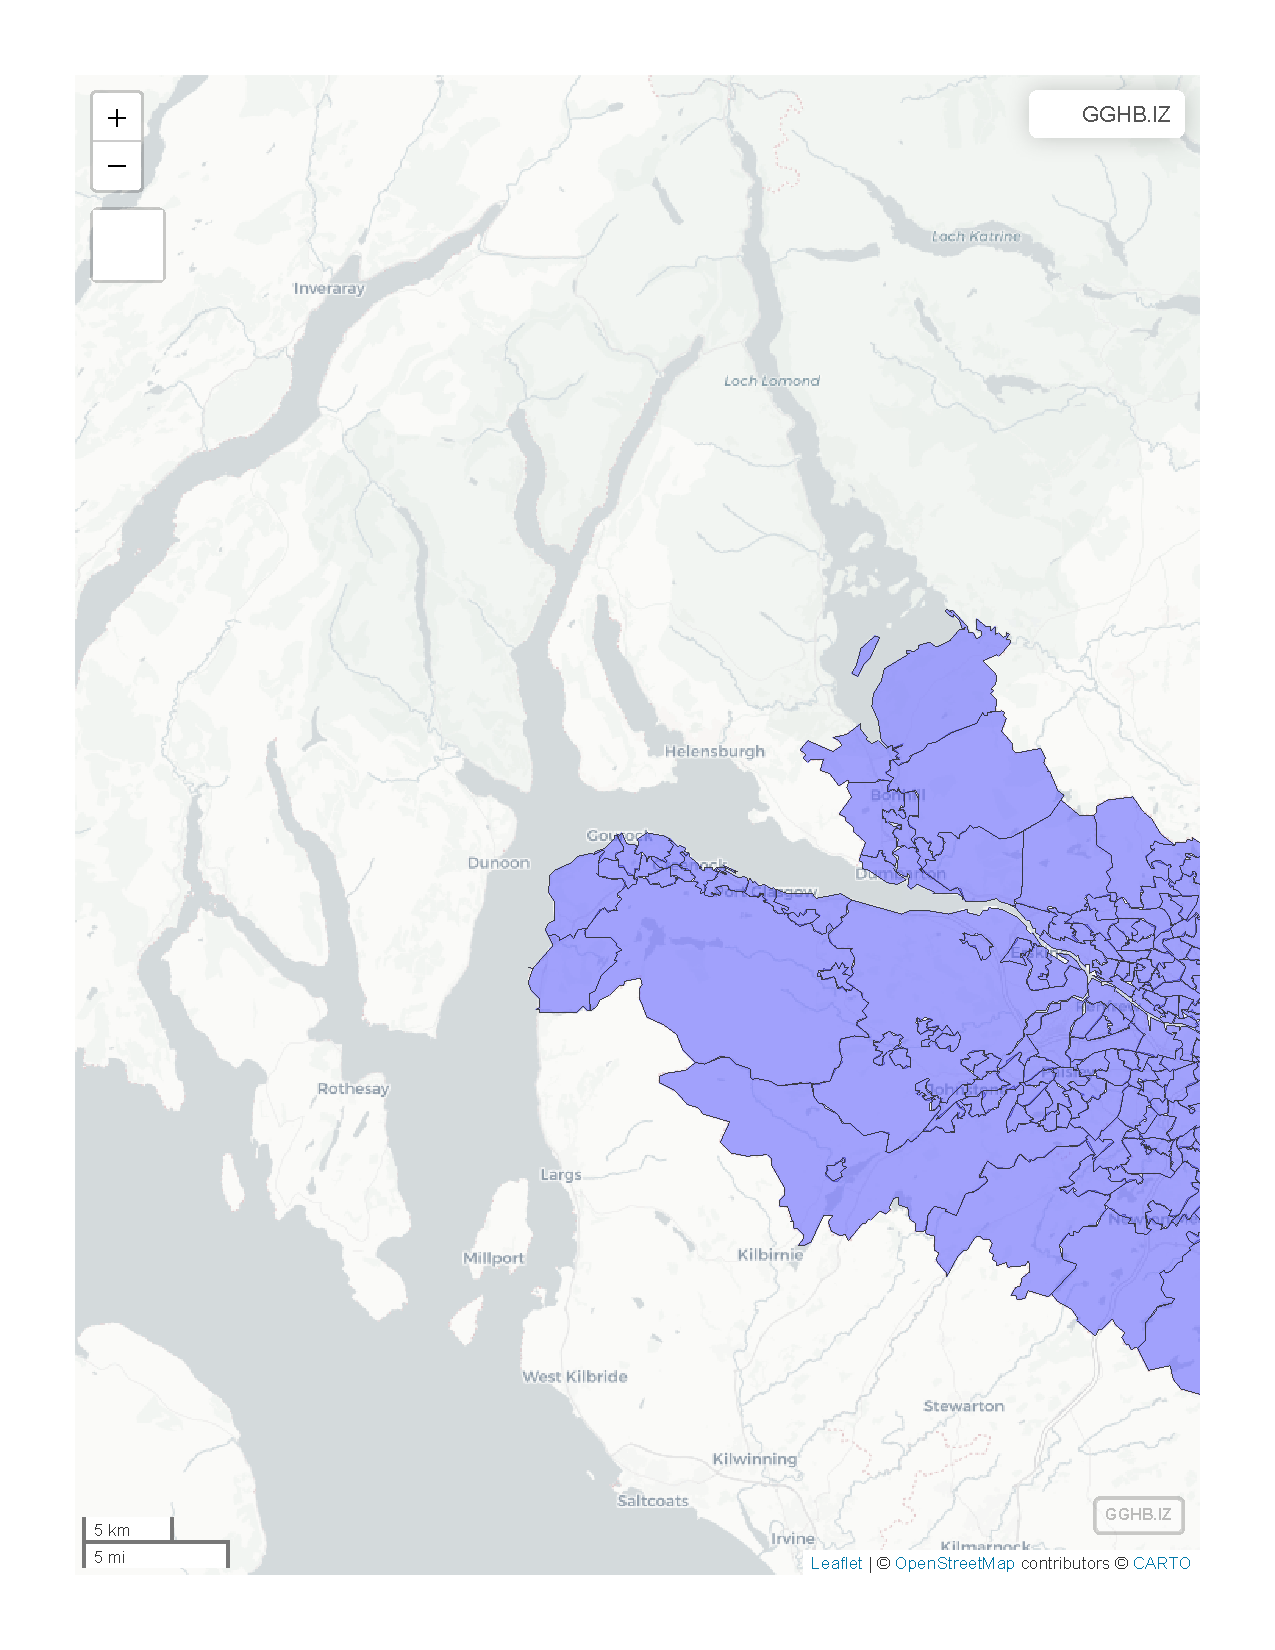
\includegraphics[keepaspectratio]{practical2_compiler_files/figure-pdf/fig-GGC-1.pdf}}

}

\caption{\label{fig-GGC}Greater Glasgow and Clyde health board
represented by 271 Intermediate Zones}

\end{figure}%

\subsubsection{Maipulating and visualizing areal
data}\label{maipulating-and-visualizing-areal-data}

Let's start by loading useful libraries:

\begin{Shaded}
\begin{Highlighting}[]
\FunctionTok{library}\NormalTok{(dplyr)}
\FunctionTok{library}\NormalTok{(INLA)}
\FunctionTok{library}\NormalTok{(ggplot2)}
\FunctionTok{library}\NormalTok{(patchwork)}
\FunctionTok{library}\NormalTok{(inlabru)   }
\FunctionTok{library}\NormalTok{(mapview)}
\FunctionTok{library}\NormalTok{(sf)}

\CommentTok{\# load some libraries to generate nice map plots}
\FunctionTok{library}\NormalTok{(scico)}
\end{Highlighting}
\end{Shaded}

The \texttt{sf} package allows us to work with vector data which is used
to represent points, lines, and polygons. It can also be used to read
vector data stored as a shapefiles.

First, lets combine both data sets based on the Intermediate Zones (IZ)
variable using the \texttt{merge} function from \texttt{base} R, and
select only one year of data

\begin{Shaded}
\begin{Highlighting}[]
\NormalTok{resp\_cases }\OtherTok{\textless{}{-}} \FunctionTok{merge}\NormalTok{(GGHB.IZ }\SpecialCharTok{\%\textgreater{}\%}
                      \FunctionTok{mutate}\NormalTok{(}\AttributeTok{space =} \DecValTok{1}\SpecialCharTok{:}\FunctionTok{dim}\NormalTok{(GGHB.IZ)[}\DecValTok{1}\NormalTok{]),}
\NormalTok{                             pollutionhealthdata, }\AttributeTok{by =} \StringTok{"IZ"}\NormalTok{)}\SpecialCharTok{\%\textgreater{}\%}
\NormalTok{  dplyr}\SpecialCharTok{::}\FunctionTok{filter}\NormalTok{(year }\SpecialCharTok{==} \DecValTok{2007}\NormalTok{) }
\end{Highlighting}
\end{Shaded}

In epidemiology, disease risk is usually estimated using Standardized
Mortality Ratios (SMR). The SMR for a given spatial areal unit \(i\) is
defined as the ratio between the observed ( \(Y_i\) ) and expected (
\(E_i\) ) number of cases:

\[
SMR_i = \dfrac{Y_i}{E_i}
\]

A value \(SMR > 1\) indicates that there are more observed cases than
expected which corresponds to a high risk area. On the other hand, if
\(SMR<1\) then there are fewer observed cases than expected, suggesting
a low risk area.

We can manipulate \texttt{sf} objects the same way we manipulate
standard data frame objects via the \texttt{dplyr} package. Lets use the
pipeline command \texttt{\%\textgreater{}\%} and the \texttt{mutate}
function to calculate the yearly SMR values for each IZ:

\begin{Shaded}
\begin{Highlighting}[]
\NormalTok{resp\_cases }\OtherTok{\textless{}{-}}\NormalTok{ resp\_cases }\SpecialCharTok{\%\textgreater{}\%} 
  \FunctionTok{mutate}\NormalTok{(}\AttributeTok{SMR =}\NormalTok{ observed}\SpecialCharTok{/}\NormalTok{expected )}
\end{Highlighting}
\end{Shaded}

Now we use \texttt{ggplot} to visualize our data by adding a
\texttt{geom\_sf} layer and coloring it according to our variable of
interest (i.e., SMR).

\begin{Shaded}
\begin{Highlighting}[]
\FunctionTok{ggplot}\NormalTok{()}\SpecialCharTok{+}
  \FunctionTok{geom\_sf}\NormalTok{(}\AttributeTok{data=}\NormalTok{resp\_cases,}\FunctionTok{aes}\NormalTok{(}\AttributeTok{fill=}\NormalTok{SMR))}\SpecialCharTok{+}
  \FunctionTok{scale\_fill\_scico}\NormalTok{(}\AttributeTok{palette =} \StringTok{"roma"}\NormalTok{)}
\end{Highlighting}
\end{Shaded}

\begin{center}
\pandocbounded{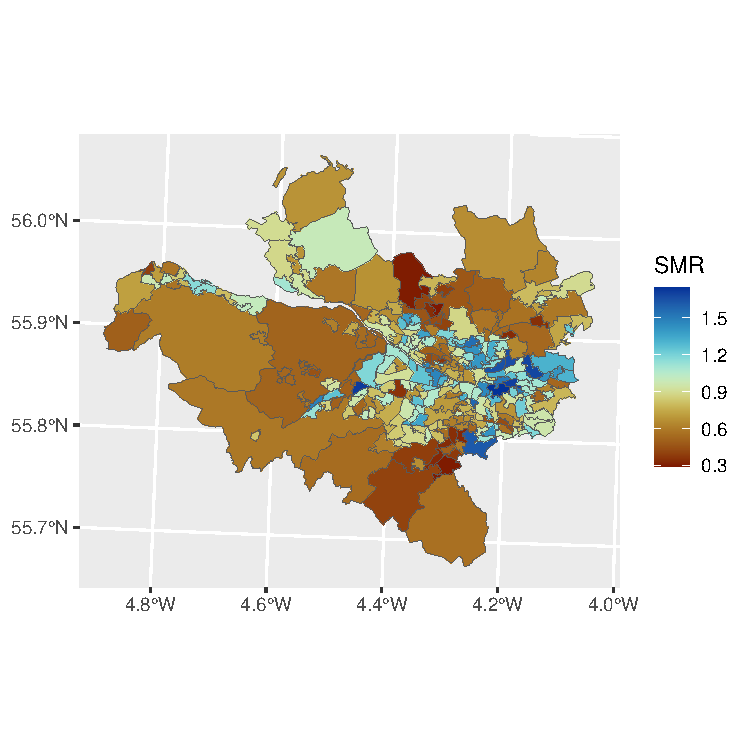
\includegraphics[keepaspectratio]{practical2_compiler_files/figure-pdf/unnamed-chunk-6-1.pdf}}
\end{center}

As with the other types of spatial modelling, our goal is to observe and
explain spatial variation in our data. Generally, we are aiming to
produce a smoothed map which summarises the spatial patterns we observe
in our data.

\subsubsection{Spatial neighbourhood
structures}\label{spatial-neighbourhood-structures}

A key aspect of any spatial analysis is that observations closer
together in space are likely to have more in common than those further
apart. This can lead us towards approaches similar to those used in time
series, where we consider the spatial \emph{closeness} of our regions in
terms of a \emph{neighbourhood structure}.

The function
\href{https://r-spatial.github.io/spdep/reference/poly2nb.html}{\texttt{poly2nb()}}
of the \texttt{spdep} package can be used to construct a list of
neighbors based on areas with contiguous boundaries (e.g., using Queen
contiguity).

\begin{Shaded}
\begin{Highlighting}[]
\FunctionTok{library}\NormalTok{(spdep)}

\NormalTok{W.nb }\OtherTok{\textless{}{-}} \FunctionTok{poly2nb}\NormalTok{(GGHB.IZ,}\AttributeTok{queen =} \ConstantTok{TRUE}\NormalTok{)}
\NormalTok{W.nb}
\end{Highlighting}
\end{Shaded}

\begin{verbatim}
Neighbour list object:
Number of regions: 271 
Number of nonzero links: 1424 
Percentage nonzero weights: 1.938971 
Average number of links: 5.254613 
2 disjoint connected subgraphs
\end{verbatim}

\begin{Shaded}
\begin{Highlighting}[]
\FunctionTok{plot}\NormalTok{(}\FunctionTok{st\_geometry}\NormalTok{(GGHB.IZ), }\AttributeTok{border =} \StringTok{"lightgray"}\NormalTok{)}
\FunctionTok{plot.nb}\NormalTok{(W.nb, }\FunctionTok{st\_geometry}\NormalTok{(GGHB.IZ), }\AttributeTok{add =} \ConstantTok{TRUE}\NormalTok{)}
\end{Highlighting}
\end{Shaded}

\begin{center}
\pandocbounded{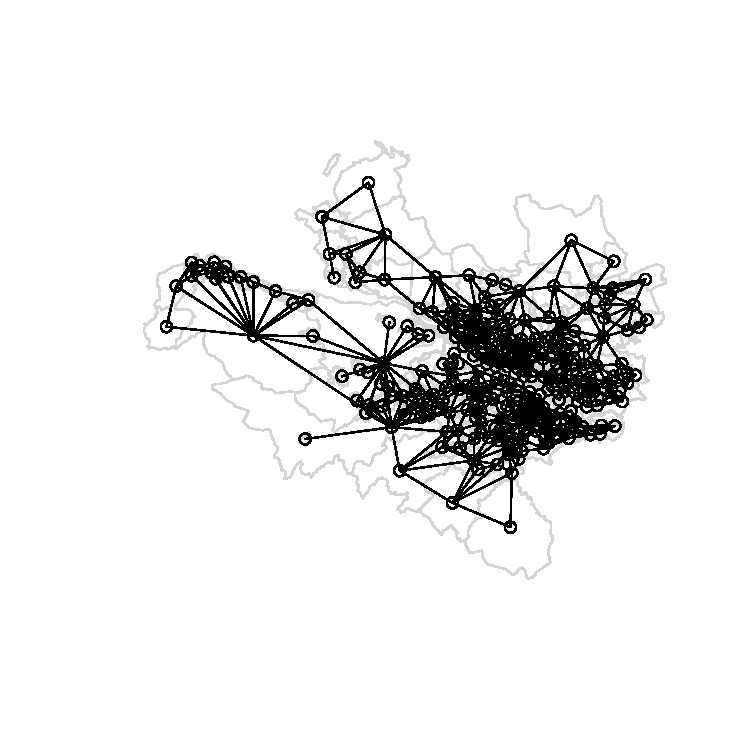
\includegraphics[keepaspectratio]{practical2_compiler_files/figure-pdf/unnamed-chunk-8-1.pdf}}
\end{center}

\begin{tcolorbox}[enhanced jigsaw, left=2mm, coltitle=black, breakable, leftrule=.75mm, colbacktitle=quarto-callout-note-color!10!white, colframe=quarto-callout-note-color-frame, rightrule=.15mm, colback=white, bottomtitle=1mm, opacitybacktitle=0.6, toptitle=1mm, titlerule=0mm, title=\textcolor{quarto-callout-note-color}{\faInfo}\hspace{0.5em}{Note}, arc=.35mm, opacityback=0, bottomrule=.15mm, toprule=.15mm]

You could use the \texttt{snap} argument within \texttt{poly2nb} to set
a distance at which the different regions centroids are consider
neighbours.

\end{tcolorbox}

With this neighborhood matrix, we can then fit a conditional
autoregressive (CAR) model. One of the most popular CAR approaches to
model spatial correlation is the Besag model a.k.a. Intrinsic
Conditional Autoregressive (ICAR) model.

The conditional distribution for \(u_i\) given
\(\mathbf{u}_{-i} = (u_i,\ldots,u_{i-1},u_{i+1},\ldots,u_n)^T\) is

\[
u_i|\mathbf{u}_{-i} \sim N\left(\frac{1}{d_i}\sum_{j\sim i}u_j,\frac{1}{d_i\tau_u}\right)
\]

where \(\tau_u\) is the precision parameter, \(j\sim i\) denotes that
\(i\) and \(j\) are neighbors, and \(d_i\) is the number of neighbors.
Thus, the mean of \(u_i\) is equivalent to the the mean of the effects
over all neighbours, and the precision is proportional to the number of
neighbors. The joint distribution is given by:

\[
\mathbf{u}|\tau_u \sim N\left(0,\frac{1}{\tau_u}Q^{-1}\right),
\]

Where \(Q\) denotes the structure matrix defined as

\[
Q_{i,j} = \begin{cases}
d_i, & i = j \\
-1, & i \sim j \\
0, &\text{otherwise}
\end{cases}
\]

This structure matrix directly defines the neighbourhood structure and
is sparse. We can compute the adjacency matrix using the function
\texttt{nb2mat()} in the \texttt{spdep} library. Then convert the
adjacency matrix into the precision matrix \(\mathbf{Q}\) of the CAR
model as follows:

\begin{Shaded}
\begin{Highlighting}[]
\FunctionTok{library}\NormalTok{(spdep)}
\NormalTok{R }\OtherTok{\textless{}{-}} \FunctionTok{nb2mat}\NormalTok{(W.nb, }\AttributeTok{style =} \StringTok{"B"}\NormalTok{, }\AttributeTok{zero.policy =} \ConstantTok{TRUE}\NormalTok{)}
\NormalTok{diag }\OtherTok{=} \FunctionTok{apply}\NormalTok{(R,}\DecValTok{1}\NormalTok{,sum)}
\NormalTok{Q }\OtherTok{=} \SpecialCharTok{{-}}\NormalTok{R}
\FunctionTok{diag}\NormalTok{(Q) }\OtherTok{=}\NormalTok{ diag}
\end{Highlighting}
\end{Shaded}

The ICAR model accounts only for spatially structured variability and
does not include a limiting case where no spatial structure is present.
Therefore, it is typically combined with an additional unstructured
random effect \(z_i|\tau_z \sim N(0,\tau_{z}^{-1})\) . The resulting
model \(v_i = u_i + z_i\) is known as the Besag-York-Mollié model (BYM)
which is an extension to the intrinsic CAR model that contains an i.i.d.
model component.

\subsubsection{\texorpdfstring{Fitting an ICAR model in
\texttt{inlabru}}{Fitting an ICAR model in inlabru}}\label{fitting-an-icar-model-in-inlabru}

We fit a first model to the data where we consider a Poisson model for
the observed cases.

\textbf{Stage 1} Model for the response \[
y_i|\eta_i\sim\text{Poisson}(E_i\lambda_i)
\] where \(E_i\) are the expected cases for area \(i\).

\textbf{Stage 2} Latent field model \[
\eta_i = \text{log}(\lambda_i) = \beta_0 + u_i + z_i
\] where

\begin{itemize}
\tightlist
\item
  \(\beta_0\) is a common intercept
\item
  \(\mathbf{u} = (u_1, \dots, u_k)\) is a conditional Autoregressive
  model (CAR) with precision matrix \(\tau_u\mathbf{Q}\)
\item
  \(\mathbf{z} = (z_1, \dots, z_k)\) is an unstructured random effect
  with precision \(\tau_z\)
\end{itemize}

\textbf{Stage 3} Hyperparameters

The hyperparameters of the model are \(\tau_u\) and \(\tau_z\)

\textbf{NOTE} In this case the linear predictor \(\eta\) consists of
three components!!

\begin{tcolorbox}[enhanced jigsaw, left=2mm, coltitle=black, breakable, leftrule=.75mm, colbacktitle=quarto-callout-tip-color!10!white, colframe=quarto-callout-tip-color-frame, rightrule=.15mm, colback=white, bottomtitle=1mm, opacitybacktitle=0.6, toptitle=1mm, titlerule=0mm, title={Question}, arc=.35mm, opacityback=0, bottomrule=.15mm, toprule=.15mm]

Fit the above model in using \texttt{inlabru} by completing the
following code:

\begin{Shaded}
\begin{Highlighting}[]
\NormalTok{cmp }\OtherTok{=} \ErrorTok{\textasciitilde{}} \FunctionTok{Intercept}\NormalTok{(}\DecValTok{1}\NormalTok{) }\SpecialCharTok{+} \FunctionTok{space}\NormalTok{(...) }\SpecialCharTok{+} \FunctionTok{iid}\NormalTok{(...)}

\NormalTok{formula }\OtherTok{=}\NormalTok{ ...}


\NormalTok{lik }\OtherTok{=} \FunctionTok{bru\_obs}\NormalTok{(}\AttributeTok{formula =}\NormalTok{ formula, }
              \AttributeTok{family =}\NormalTok{ ...,}
              \AttributeTok{E =}\NormalTok{ ...,}
              \AttributeTok{data =}\NormalTok{ ...)}

\NormalTok{fit }\OtherTok{=} \FunctionTok{bru}\NormalTok{(cmp, lik)}
\end{Highlighting}
\end{Shaded}

Answer

\begin{Shaded}
\begin{Highlighting}[]
\NormalTok{cmp }\OtherTok{=} \ErrorTok{\textasciitilde{}} \FunctionTok{Intercept}\NormalTok{(}\DecValTok{1}\NormalTok{) }\SpecialCharTok{+} \FunctionTok{space}\NormalTok{(space, }\AttributeTok{model =} \StringTok{"besag"}\NormalTok{, }\AttributeTok{graph =}\NormalTok{ Q) }\SpecialCharTok{+} \FunctionTok{iid}\NormalTok{(space, }\AttributeTok{model =} \StringTok{"iid"}\NormalTok{)}

\NormalTok{formula }\OtherTok{=}\NormalTok{ observed }\SpecialCharTok{\textasciitilde{}}\NormalTok{ Intercept }\SpecialCharTok{+}\NormalTok{ space }\SpecialCharTok{+}\NormalTok{ iid}

\NormalTok{lik }\OtherTok{=} \FunctionTok{bru\_obs}\NormalTok{(}\AttributeTok{formula =}\NormalTok{ formula, }
              \AttributeTok{family =} \StringTok{"poisson"}\NormalTok{,}
              \AttributeTok{E =}\NormalTok{ expected,}
              \AttributeTok{data =}\NormalTok{ resp\_cases)}

\NormalTok{fit }\OtherTok{=} \FunctionTok{bru}\NormalTok{(cmp, lik)}
\end{Highlighting}
\end{Shaded}

\end{tcolorbox}

After fitting the model we want to extract results.

\begin{tcolorbox}[enhanced jigsaw, left=2mm, coltitle=black, breakable, leftrule=.75mm, colbacktitle=quarto-callout-tip-color!10!white, colframe=quarto-callout-tip-color-frame, rightrule=.15mm, colback=white, bottomtitle=1mm, opacitybacktitle=0.6, toptitle=1mm, titlerule=0mm, title={Question}, arc=.35mm, opacityback=0, bottomrule=.15mm, toprule=.15mm]

\begin{enumerate}
\def\labelenumi{\arabic{enumi}.}
\item
  What is the estimated value for \(\beta_0\)?
\item
  Look at the estimated values of the hyperparameters using
\end{enumerate}

\begin{Shaded}
\begin{Highlighting}[]
\NormalTok{fit}\SpecialCharTok{$}\NormalTok{summary.hyperpar}
\end{Highlighting}
\end{Shaded}

Which of the two spatial components (structured or unstructured)
explains more of the variability in the counts?

\end{tcolorbox}

\subsubsection{Areal model predictions}\label{areal-model-predictions}

We now look at the predictions over space.

\begin{tcolorbox}[enhanced jigsaw, left=2mm, coltitle=black, breakable, leftrule=.75mm, colbacktitle=quarto-callout-warning-color!10!white, colframe=quarto-callout-warning-color-frame, rightrule=.15mm, colback=white, bottomtitle=1mm, opacitybacktitle=0.6, toptitle=1mm, titlerule=0mm, title={Task}, arc=.35mm, opacityback=0, bottomrule=.15mm, toprule=.15mm]

Complete the code below to produce:

\begin{enumerate}
\def\labelenumi{\arabic{enumi}.}
\item
  prediction of the linear predictor \(\eta_i\)
\item
  The risk rate \(\lambda_i\)
\item
  The expected cases \(E_i\exp(\lambda_i)\) over the whole space of
  interest.
\end{enumerate}

Plot the mean and sd of the resulting surfaces.

\begin{Shaded}
\begin{Highlighting}[]
\NormalTok{pred }\OtherTok{=} \FunctionTok{predict}\NormalTok{(fit, resp\_cases, }\SpecialCharTok{\textasciitilde{}}\FunctionTok{data.frame}\NormalTok{(}\AttributeTok{log\_risk =}\NormalTok{ ...,}
                                             \AttributeTok{risk =} \FunctionTok{exp}\NormalTok{(...),}
                                             \AttributeTok{cases =}\NormalTok{ ...}
\NormalTok{                                             ),}
               \AttributeTok{n.samples =} \DecValTok{1000}\NormalTok{)}
\end{Highlighting}
\end{Shaded}

See Solution

\begin{Shaded}
\begin{Highlighting}[]
\CommentTok{\# produce predictions}
\NormalTok{pred }\OtherTok{=} \FunctionTok{predict}\NormalTok{(fit, }
\NormalTok{               resp\_cases,}
               \SpecialCharTok{\textasciitilde{}}\FunctionTok{data.frame}\NormalTok{(}\AttributeTok{log\_risk =}\NormalTok{ Intercept }\SpecialCharTok{+}\NormalTok{ space,}
                           \AttributeTok{risk =} \FunctionTok{exp}\NormalTok{(Intercept }\SpecialCharTok{+}\NormalTok{ space),}
                           \AttributeTok{cases =}\NormalTok{ expected }\SpecialCharTok{*} \FunctionTok{exp}\NormalTok{(Intercept }\SpecialCharTok{+}\NormalTok{ space)),}
               \AttributeTok{n.samples =} \DecValTok{1000}\NormalTok{)}

\CommentTok{\# plot the predictions}

\NormalTok{p1 }\OtherTok{=} \FunctionTok{ggplot}\NormalTok{() }\SpecialCharTok{+} 
  \FunctionTok{geom\_sf}\NormalTok{(}\AttributeTok{data =}\NormalTok{ pred}\SpecialCharTok{$}\NormalTok{log\_risk, }\FunctionTok{aes}\NormalTok{(}\AttributeTok{fill =}\NormalTok{ mean)) }\SpecialCharTok{+} \FunctionTok{scale\_fill\_scico}\NormalTok{(}\AttributeTok{direction =} \SpecialCharTok{{-}}\DecValTok{1}\NormalTok{) }\SpecialCharTok{+}
  \FunctionTok{ggtitle}\NormalTok{(}\StringTok{"mean log risk"}\NormalTok{)}
\NormalTok{p2 }\OtherTok{=} \FunctionTok{ggplot}\NormalTok{() }\SpecialCharTok{+} 
  \FunctionTok{geom\_sf}\NormalTok{(}\AttributeTok{data =}\NormalTok{ pred}\SpecialCharTok{$}\NormalTok{log\_risk, }\FunctionTok{aes}\NormalTok{(}\AttributeTok{fill =}\NormalTok{ sd)) }\SpecialCharTok{+} \FunctionTok{scale\_fill\_scico}\NormalTok{(}\AttributeTok{direction =} \SpecialCharTok{{-}}\DecValTok{1}\NormalTok{) }\SpecialCharTok{+}
  \FunctionTok{ggtitle}\NormalTok{(}\StringTok{"sd log risk"}\NormalTok{)}

\NormalTok{p3 }\OtherTok{=} \FunctionTok{ggplot}\NormalTok{() }\SpecialCharTok{+}
  \FunctionTok{geom\_sf}\NormalTok{(}\AttributeTok{data =}\NormalTok{ pred}\SpecialCharTok{$}\NormalTok{risk, }\FunctionTok{aes}\NormalTok{(}\AttributeTok{fill =}\NormalTok{ mean)) }\SpecialCharTok{+} \FunctionTok{scale\_fill\_scico}\NormalTok{(}\AttributeTok{direction =} \SpecialCharTok{{-}}\DecValTok{1}\NormalTok{) }\SpecialCharTok{+}
  \FunctionTok{ggtitle}\NormalTok{(}\StringTok{"mean  risk"}\NormalTok{)}

\NormalTok{p4 }\OtherTok{=} \FunctionTok{ggplot}\NormalTok{() }\SpecialCharTok{+} 
  \FunctionTok{geom\_sf}\NormalTok{(}\AttributeTok{data =}\NormalTok{ pred}\SpecialCharTok{$}\NormalTok{risk, }\FunctionTok{aes}\NormalTok{(}\AttributeTok{fill =}\NormalTok{ sd)) }\SpecialCharTok{+}
  \FunctionTok{scale\_fill\_scico}\NormalTok{(}\AttributeTok{direction =} \SpecialCharTok{{-}}\DecValTok{1}\NormalTok{) }\SpecialCharTok{+}
  \FunctionTok{ggtitle}\NormalTok{(}\StringTok{"sd  risk"}\NormalTok{)}

\NormalTok{p5 }\OtherTok{=} \FunctionTok{ggplot}\NormalTok{() }\SpecialCharTok{+} \FunctionTok{geom\_sf}\NormalTok{(}\AttributeTok{data =}\NormalTok{ pred}\SpecialCharTok{$}\NormalTok{cases, }\FunctionTok{aes}\NormalTok{(}\AttributeTok{fill =}\NormalTok{ mean)) }\SpecialCharTok{+} \FunctionTok{scale\_fill\_scico}\NormalTok{(}\AttributeTok{direction =} \SpecialCharTok{{-}}\DecValTok{1}\NormalTok{)}\SpecialCharTok{+} 
  \FunctionTok{ggtitle}\NormalTok{(}\StringTok{"mean  expected counts"}\NormalTok{)}
\NormalTok{p6 }\OtherTok{=} \FunctionTok{ggplot}\NormalTok{() }\SpecialCharTok{+} \FunctionTok{geom\_sf}\NormalTok{(}\AttributeTok{data =}\NormalTok{ pred}\SpecialCharTok{$}\NormalTok{cases, }\FunctionTok{aes}\NormalTok{(}\AttributeTok{fill =}\NormalTok{ sd)) }\SpecialCharTok{+} \FunctionTok{scale\_fill\_scico}\NormalTok{(}\AttributeTok{direction =} \SpecialCharTok{{-}}\DecValTok{1}\NormalTok{)}\SpecialCharTok{+}
  \FunctionTok{ggtitle}\NormalTok{(}\StringTok{"sd  expected counts"}\NormalTok{)}

\NormalTok{p1 }\SpecialCharTok{+}\NormalTok{ p2 }\SpecialCharTok{+}\NormalTok{ p3 }\SpecialCharTok{+}\NormalTok{ p4 }\SpecialCharTok{+}\NormalTok{p5 }\SpecialCharTok{+}\NormalTok{ p6 }\SpecialCharTok{+} \FunctionTok{plot\_layout}\NormalTok{(}\AttributeTok{ncol=}\DecValTok{2}\NormalTok{)}
\end{Highlighting}
\end{Shaded}

\pandocbounded{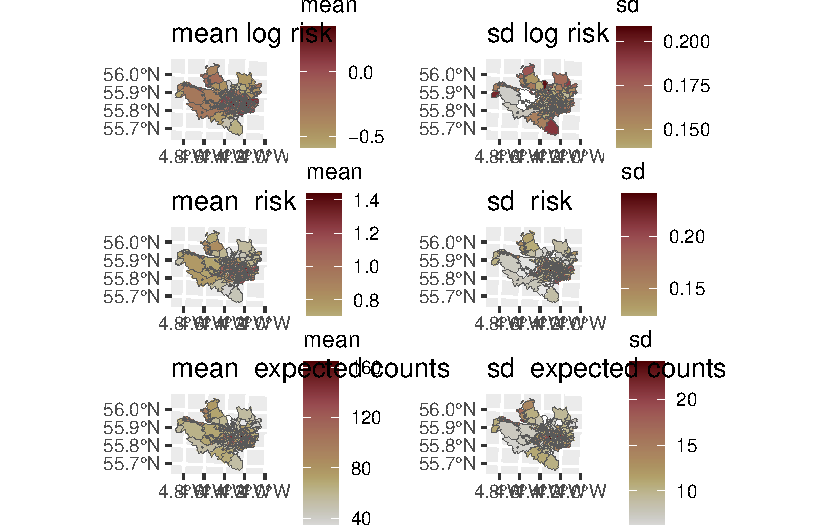
\includegraphics[keepaspectratio]{practical2_compiler_files/figure-pdf/unnamed-chunk-14-1.pdf}}

\end{tcolorbox}

Finally we want to compare our observations \(y_i\) with the predicted
means of the Poisson distribution \(E_i\exp(\lambda_i)\)

\begin{Shaded}
\begin{Highlighting}[]
\NormalTok{pred}\SpecialCharTok{$}\NormalTok{cases }\SpecialCharTok{\%\textgreater{}\%} \FunctionTok{ggplot}\NormalTok{() }\SpecialCharTok{+} \FunctionTok{geom\_point}\NormalTok{(}\FunctionTok{aes}\NormalTok{(observed, mean)) }\SpecialCharTok{+} 
  \FunctionTok{geom\_errorbar}\NormalTok{(}\FunctionTok{aes}\NormalTok{(observed, }\AttributeTok{ymin =}\NormalTok{ q0}\FloatTok{.025}\NormalTok{, }\AttributeTok{ymax =}\NormalTok{ q0}\FloatTok{.975}\NormalTok{)) }\SpecialCharTok{+}
  \FunctionTok{geom\_abline}\NormalTok{(}\AttributeTok{intercept =} \DecValTok{0}\NormalTok{, }\AttributeTok{slope =} \DecValTok{1}\NormalTok{)}
\end{Highlighting}
\end{Shaded}

\begin{center}
\pandocbounded{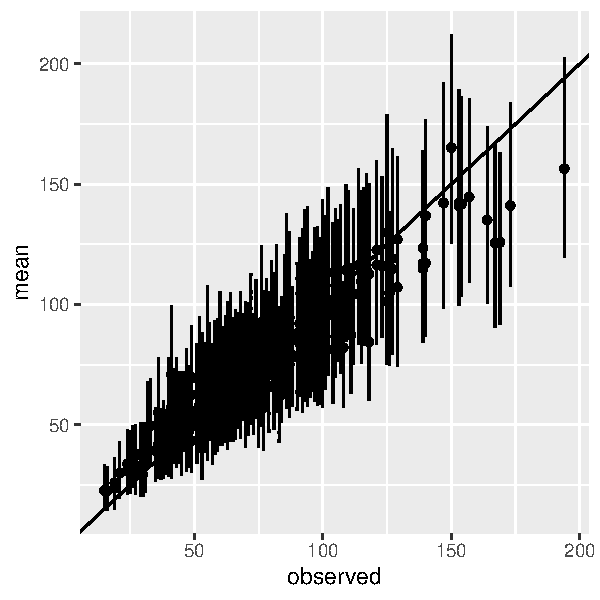
\includegraphics[keepaspectratio]{practical2_compiler_files/figure-pdf/unnamed-chunk-15-1.pdf}}
\end{center}

Here we are predicting the \emph{mean} of counts, not the counts.
Predicting the counts is beyond the scope of this short course but you
can check the supplementary material below.

\begin{tcolorbox}[enhanced jigsaw, left=2mm, breakable, leftrule=.75mm, arc=.35mm, bottomrule=.15mm, colframe=quarto-callout-note-color-frame, rightrule=.15mm, opacityback=0, colback=white, toprule=.15mm]

\vspace{-3mm}\textbf{Supplementary Material}\vspace{3mm}

Posterior predictive distributions, i.e.,
\(\pi(y_i^{\text{new}}|\mathbf{y})\) are of interest in many applied
problems. The \texttt{bru()} function does not return predictive
densities. In the previous step we have computed predictions for the
\texttt{expected\ counts} \(\pi(E_i\lambda_i|\mathbf{y})\).

The predictive distribution is then: \[
\pi(y_i^{\text{new}}|\mathbf{y}) = \int \pi(y_i|E_i\lambda_i)\pi(E_i\lambda_i|\mathbf{y})\ dE_i\lambda_i
\] where, in our case, \(\pi(y_i|E_i\lambda_i)\) is Poisson with mean
\(E_i\lambda_i\). We can achieve this using the following algorithm:

\begin{enumerate}
\def\labelenumi{\arabic{enumi}.}
\tightlist
\item
  Simulate \(n\) replicates of \(g^k = E_i\lambda_i\) for
  \(k = 1,\dots,n\) using the function \texttt{generate()} which takes
  the same input as \texttt{predict()}
\item
  For each of the \(k\) replicates simulate a new value \(y_i^{new}\)
  using the function \texttt{rpois()}
\item
  Summarise the \(n\) samples of \(y_i^{new}\) using, for example the
  mean and the 0.025 and 0.975 quantiles.
\item
\end{enumerate}

\begin{Shaded}
\begin{Highlighting}[]
\CommentTok{\# simulate 1000 realizations of E\_i\textbackslash{}lambda\_i}
\NormalTok{expected\_counts }\OtherTok{=} \FunctionTok{generate}\NormalTok{(fit, resp\_cases, }
                           \SpecialCharTok{\textasciitilde{}}\NormalTok{ expected }\SpecialCharTok{*} \FunctionTok{exp}\NormalTok{(Intercept }\SpecialCharTok{+}\NormalTok{ space),}
                           \AttributeTok{n.samples =} \DecValTok{1000}\NormalTok{)}


\CommentTok{\# simulate poisson data}
\NormalTok{aa }\OtherTok{=} \FunctionTok{rpois}\NormalTok{(}\DecValTok{271}\SpecialCharTok{*}\DecValTok{1000}\NormalTok{, }\AttributeTok{lambda =} \FunctionTok{as.vector}\NormalTok{(expected\_counts))}
\NormalTok{sim\_counts }\OtherTok{=} \FunctionTok{matrix}\NormalTok{(aa, }\DecValTok{271}\NormalTok{, }\DecValTok{1000}\NormalTok{)}

\CommentTok{\# summarise the samples with posterior means and quantiles}
\NormalTok{pred\_counts }\OtherTok{=} \FunctionTok{data.frame}\NormalTok{(}\AttributeTok{observed =}\NormalTok{ resp\_cases}\SpecialCharTok{$}\NormalTok{observed,}
                         \AttributeTok{m =} \FunctionTok{apply}\NormalTok{(sim\_counts,}\DecValTok{1}\NormalTok{,mean),}
                         \AttributeTok{q1 =} \FunctionTok{apply}\NormalTok{(sim\_counts,}\DecValTok{1}\NormalTok{,quantile, }\FloatTok{0.025}\NormalTok{),}
                         \AttributeTok{q2 =} \FunctionTok{apply}\NormalTok{(sim\_counts,}\DecValTok{1}\NormalTok{,quantile, }\FloatTok{0.975}\NormalTok{),}
                         \AttributeTok{vv =} \FunctionTok{apply}\NormalTok{(sim\_counts,}\DecValTok{1}\NormalTok{,var)}
\NormalTok{                         )}
\CommentTok{\# Plot the observations against the predicted new counts and the predicted expected counts}

\FunctionTok{ggplot}\NormalTok{() }\SpecialCharTok{+} 
  \FunctionTok{geom\_point}\NormalTok{(}\AttributeTok{data =}\NormalTok{ pred\_counts, }\FunctionTok{aes}\NormalTok{(observed, m, }\AttributeTok{color =} \StringTok{"Pred\_obs"}\NormalTok{)) }\SpecialCharTok{+} 
  \FunctionTok{geom\_errorbar}\NormalTok{(}\AttributeTok{data =}\NormalTok{ pred\_counts, }\FunctionTok{aes}\NormalTok{(observed, }\AttributeTok{ymin =}\NormalTok{ q1, }\AttributeTok{ymax =}\NormalTok{ q2, }\AttributeTok{color =} \StringTok{"Pred\_obs"}\NormalTok{)) }\SpecialCharTok{+}
  \FunctionTok{geom\_point}\NormalTok{(}\AttributeTok{data =}\NormalTok{ pred}\SpecialCharTok{$}\NormalTok{cases, }\FunctionTok{aes}\NormalTok{(observed, mean, }\AttributeTok{color =} \StringTok{"Pred\_means"}\NormalTok{)) }\SpecialCharTok{+} 
  \FunctionTok{geom\_errorbar}\NormalTok{(}\AttributeTok{data =}\NormalTok{ pred}\SpecialCharTok{$}\NormalTok{cases, }\FunctionTok{aes}\NormalTok{(observed, }\AttributeTok{ymin =}\NormalTok{ q0}\FloatTok{.025}\NormalTok{, }\AttributeTok{ymax =}\NormalTok{ q0}\FloatTok{.975}\NormalTok{, }\AttributeTok{color =} \StringTok{"Pred\_means"}\NormalTok{)) }\SpecialCharTok{+}
  
  \FunctionTok{geom\_abline}\NormalTok{(}\AttributeTok{intercept =} \DecValTok{0}\NormalTok{, }\AttributeTok{slope =}\DecValTok{1}\NormalTok{)}
\end{Highlighting}
\end{Shaded}

\begin{center}
\pandocbounded{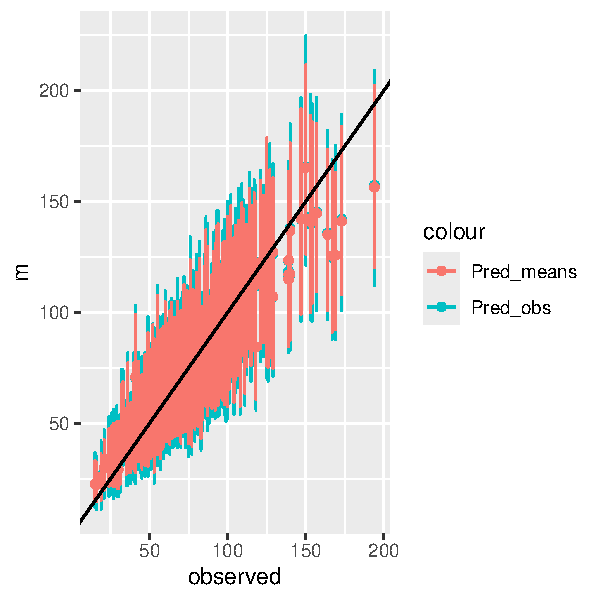
\includegraphics[keepaspectratio]{practical2_compiler_files/figure-pdf/unnamed-chunk-16-1.pdf}}
\end{center}

\end{tcolorbox}

\subsection{Geostatistical data}\label{geostatistical-data}

In this practical we are going to fit a geostatistical model. We will:

\begin{itemize}
\item
  Explore tools for geostatistical spatial data wrangling and
  visualization.
\item
  Learn how to fit a geostatistical model in \texttt{inlabru}
\item
  Learn how to add spatial covariates to the model
\item
  Learn how to do predictions
\end{itemize}

\textbf{Geostatistical} data are the most common form of spatial data
found in environmental setting. In these data we regularly take
measurements of a spatial ecological or environmental process at a set
of fixed locations. This could be data from transects (e.g, where the
height of trees is recorded), samples taken across a region (e.g., water
depth in a lake) or from monitoring stations as part of a network (e.g.,
air pollution). In each of these cases, our goal is to estimate the
value of our variable across the entire space.

Let \(D\) be our two-dimensional region of interest. In principle, there
are infinite locations within \(D\), each of which can be represented by
mathematical coordinates (e.g., latitude and longitude). We then can
identify any individual location as \(s_i = (x_i, y_i)\), where \(x_i\)
and \(y_i\) are their coordinates.

We can treat our variable of interest as a random variable, \(Z\) which
can be observed at any location as \(Z(\mathbf{s}_i)\).

Our geostatistical process can therefore be written as:
\[\{Z(\mathbf{s}); \mathbf{s} \in D\}\]

In practice, our data are observed at a finite number of locations,
\(m\), and can be denoted as:

\[z = \{z(\mathbf{s}_1), \ldots z(\mathbf{s}_m) \}\]

In the next example, we will explore data on the Pacific Cod
(\emph{Gadus macrocephalus}) from a trawl survey in Queen Charlotte
Sound. The \texttt{pcod} dataset is available from the \texttt{sdmTMB}
package and contains the presence/absence records of the Pacific Cod
during each survey. The \texttt{qcs\_grid} data contain the depth values
stored as \(2\times 2\) km grid for Queen Charlotte Sound.

\subsubsection{Exploring and visualizing species distribution
data}\label{exploring-and-visualizing-species-distribution-data}

The dataset contains presence/absence data from 2003 to 2017. In this
practical we only consider year 2003. We first load the dataset and
select the year of interest:

\begin{Shaded}
\begin{Highlighting}[]
\FunctionTok{library}\NormalTok{(sdmTMB)}

\NormalTok{pcod\_df }\OtherTok{=}\NormalTok{ sdmTMB}\SpecialCharTok{::}\NormalTok{pcod }\SpecialCharTok{\%\textgreater{}\%} \FunctionTok{filter}\NormalTok{(year}\SpecialCharTok{==}\DecValTok{2003}\NormalTok{)}
\NormalTok{qcs\_grid }\OtherTok{=}\NormalTok{ sdmTMB}\SpecialCharTok{::}\NormalTok{qcs\_grid}
\end{Highlighting}
\end{Shaded}

Then, we create an \texttt{sf} object and assign the rough coordinate
reference to it:

\begin{Shaded}
\begin{Highlighting}[]
\NormalTok{pcod\_sf }\OtherTok{=}   \FunctionTok{st\_as\_sf}\NormalTok{(pcod\_df, }\AttributeTok{coords =} \FunctionTok{c}\NormalTok{(}\StringTok{"lon"}\NormalTok{,}\StringTok{"lat"}\NormalTok{), }\AttributeTok{crs =} \DecValTok{4326}\NormalTok{)}
\NormalTok{pcod\_sf }\OtherTok{=} \FunctionTok{st\_transform}\NormalTok{(pcod\_sf,}
                       \AttributeTok{crs =} \StringTok{"+proj=utm +zone=9 +datum=WGS84 +no\_defs +type=crs +units=km"}\NormalTok{ )}
\end{Highlighting}
\end{Shaded}

We convert the covariate into a raster and assign the same coordinate
reference:

\begin{Shaded}
\begin{Highlighting}[]
\FunctionTok{library}\NormalTok{(terra)}
\NormalTok{depth\_r }\OtherTok{\textless{}{-}} \FunctionTok{rast}\NormalTok{(qcs\_grid, }\AttributeTok{type =} \StringTok{"xyz"}\NormalTok{)}
\FunctionTok{crs}\NormalTok{(depth\_r) }\OtherTok{\textless{}{-}} \FunctionTok{crs}\NormalTok{(pcod\_sf)}
\end{Highlighting}
\end{Shaded}

Finally we can plot our dataset. Note that to plot the raster we need to
load also the \texttt{tidyterra} library.

\begin{Shaded}
\begin{Highlighting}[]
\FunctionTok{library}\NormalTok{(tidyterra)}
\FunctionTok{ggplot}\NormalTok{()}\SpecialCharTok{+} 
  \FunctionTok{geom\_spatraster}\NormalTok{(}\AttributeTok{data=}\NormalTok{depth\_r}\SpecialCharTok{$}\NormalTok{depth)}\SpecialCharTok{+}
  \FunctionTok{geom\_sf}\NormalTok{(}\AttributeTok{data=}\NormalTok{pcod\_sf,}\FunctionTok{aes}\NormalTok{(}\AttributeTok{color=}\FunctionTok{factor}\NormalTok{(present))) }\SpecialCharTok{+}
    \FunctionTok{scale\_color\_manual}\NormalTok{(}\AttributeTok{name=}\StringTok{"Occupancy status for the Pacific Cod"}\NormalTok{,}
                     \AttributeTok{values =} \FunctionTok{c}\NormalTok{(}\StringTok{"black"}\NormalTok{,}\StringTok{"orange"}\NormalTok{),}
                     \AttributeTok{labels=} \FunctionTok{c}\NormalTok{(}\StringTok{"Absence"}\NormalTok{,}\StringTok{"Presence"}\NormalTok{))}\SpecialCharTok{+}
  \FunctionTok{scale\_fill\_scico}\NormalTok{(}\AttributeTok{name =} \StringTok{"Depth"}\NormalTok{,}
                   \AttributeTok{palette =} \StringTok{"nuuk"}\NormalTok{,}
                   \AttributeTok{na.value =} \StringTok{"transparent"}\NormalTok{ ) }\SpecialCharTok{+} \FunctionTok{xlab}\NormalTok{(}\StringTok{""}\NormalTok{) }\SpecialCharTok{+} \FunctionTok{ylab}\NormalTok{(}\StringTok{""}\NormalTok{)}
\end{Highlighting}
\end{Shaded}

\begin{center}
\pandocbounded{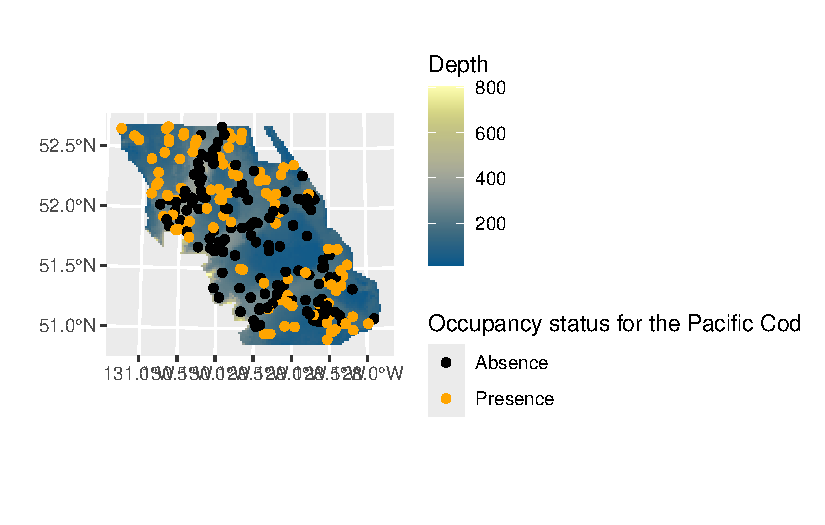
\includegraphics[keepaspectratio]{practical2_compiler_files/figure-pdf/unnamed-chunk-40-1.pdf}}
\end{center}

\subsubsection{Fitting a spatial geostatistical species distribution
model}\label{fitting-a-spatial-geostatistical-species-distribution-model}

We first fit a simple model where we consider the observation as
Bernoulli and where the linear predictor contains only one intercept and
the GR field defined through the SPDE approach. The model is defined as:

\textbf{Stage 1} Model for the response

\[
y(s)|\eta(s)\sim\text{Binom}(1, p(s))
\] \textbf{Stage 2} Latent field model

\[
\eta(s) = \text{logit}(p(s)) = \beta_0 + \omega(s)
\]

with

\[
\omega(s)\sim \text{  GF with range } \rho\  \text{ and maginal variance }\ \sigma^2
\]

\textbf{Stage 3} Hyperparameters

The hyperparameters of the model are \(\rho\) and \(\sigma\)

\textbf{NOTE} In this case the linear predictor \(\eta\) consists of two
components!!

\subsubsection{The workflow}\label{the-workflow}

When fitting a geostatistical model we need to fulfill the following
tasks:

\begin{enumerate}
\def\labelenumi{\arabic{enumi}.}
\tightlist
\item
  Build the mesh
\item
  Define the SPDE representation of the spatial GF. This includes
  defining the priors for the range and sd of the spatial GF
\item
  Define the \emph{components} of the linear predictor. This includes
  the spatial GF and all eventual covariates
\item
  Define the observation model using the \texttt{bru\_obs()} function
\item
  Run the model using the \texttt{bru()} function
\end{enumerate}

\paragraph{Step 1. Building the mesh}\label{step-1.-building-the-mesh}

The first task, when dealing with geostatistical models in
\texttt{inlabru} is to build the mesh that covers the area of interest.
For this purpose we use the function \texttt{fm\_mesh\_2d}.

One way to build the mesh is to start from the locations where we have
observations, these are contained in the dataset \texttt{pcod\_sf}

\begin{Shaded}
\begin{Highlighting}[]
\NormalTok{mesh }\OtherTok{=} \FunctionTok{fm\_mesh\_2d}\NormalTok{(}\AttributeTok{loc =}\NormalTok{ pcod\_sf,           }\CommentTok{\# Build the mesh}
                  \AttributeTok{cutoff =} \DecValTok{2}\NormalTok{,}
                  \AttributeTok{max.edge =} \FunctionTok{c}\NormalTok{(}\DecValTok{7}\NormalTok{,}\DecValTok{20}\NormalTok{),     }\CommentTok{\# The largest allowed triangle edge length.}
                  \AttributeTok{offset =} \FunctionTok{c}\NormalTok{(}\DecValTok{5}\NormalTok{,}\DecValTok{50}\NormalTok{))       }\CommentTok{\# The automatic extension distance}

\FunctionTok{ggplot}\NormalTok{() }\SpecialCharTok{+} \FunctionTok{gg}\NormalTok{(mesh) }\SpecialCharTok{+}
  \FunctionTok{geom\_sf}\NormalTok{(}\AttributeTok{data=}\NormalTok{ pcod\_sf, }\FunctionTok{aes}\NormalTok{(}\AttributeTok{color =} \FunctionTok{factor}\NormalTok{(present))) }\SpecialCharTok{+} 
  \FunctionTok{xlab}\NormalTok{(}\StringTok{""}\NormalTok{) }\SpecialCharTok{+} \FunctionTok{ylab}\NormalTok{(}\StringTok{""}\NormalTok{)}
\end{Highlighting}
\end{Shaded}

\begin{center}
\pandocbounded{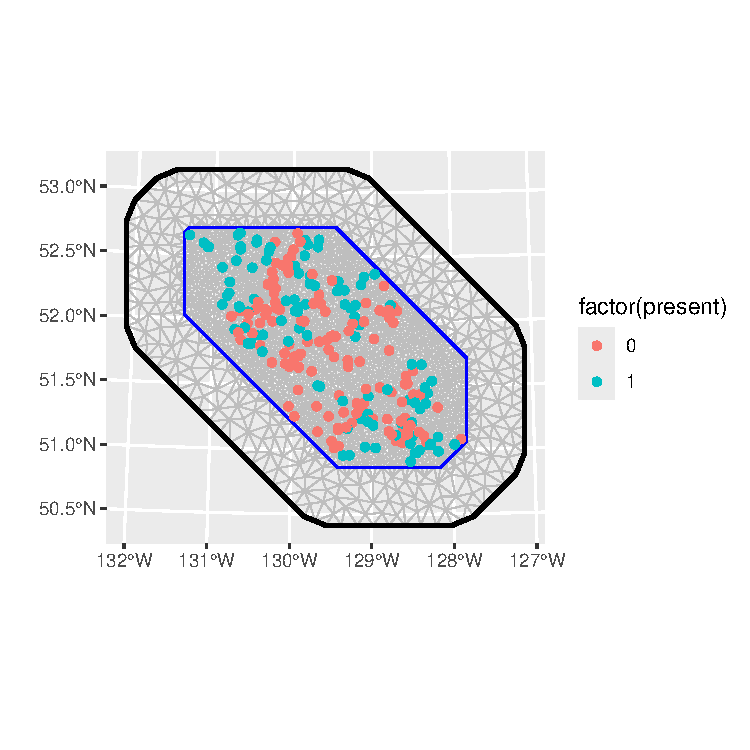
\includegraphics[keepaspectratio]{practical2_compiler_files/figure-pdf/unnamed-chunk-41-1.pdf}}
\end{center}

\begin{tcolorbox}[enhanced jigsaw, left=2mm, coltitle=black, breakable, leftrule=.75mm, colbacktitle=quarto-callout-warning-color!10!white, colframe=quarto-callout-warning-color-frame, rightrule=.15mm, colback=white, bottomtitle=1mm, opacitybacktitle=0.6, toptitle=1mm, titlerule=0mm, title={Task}, arc=.35mm, opacityback=0, bottomrule=.15mm, toprule=.15mm]

Look at the documentation for the \texttt{fm\_mesh\_2d} function typing

\begin{Shaded}
\begin{Highlighting}[]
\NormalTok{?fm\_mesh\_2d}
\end{Highlighting}
\end{Shaded}

Experiment with the different options and create different meshes (see
\href{https://ecol-stats.github.io/Spatial_Data_Analysis/\#building-a-mesh-with-fmesher}{here}
for further details on mesh construction).

The \emph{rule of thumb} is that your mesh should be:

\begin{itemize}
\tightlist
\item
  fine enough to well represent the spatial variability of your process,
  but not too fine in order to avoid computation burden
\item
  the triangles should be regular, avoid long and thin triangles.
\item
  The mesh should contain a buffer around your area of interest (this is
  what is defined in the \texttt{offset} option) in order to avoid
  boundary artifact in the estimated variance.
\end{itemize}

\end{tcolorbox}

\paragraph{Step 2. Define the SPDE representation of the spatial
GF}\label{step-2.-define-the-spde-representation-of-the-spatial-gf}

To define the SPDE representation of the spatial GF we use the function
\texttt{inla.spde2.pcmatern}.

This takes as input the mesh we have defined and the PC-priors
definition for \(\rho\) and \(\sigma\) (the range and the marginal
standard deviation of the field).

PC priors Gaussian Random field are defined in (Fuglstad et al.~2018).
From a practical perspective for the range \(\rho\) you need to define
two parameters \(\rho_0\) and \(p_{\rho}\) such that you believe it is
reasonable that

\[
P(\rho<\rho_0)=p_{\rho}
\]

while for the marginal variance \(\sigma\) you need to define two
parameters \(\sigma_0\) and \(p_{\sigma}\) such that you believe it is
reasonable that

\[
P(\sigma>\sigma_0)=p_{\sigma}
\] Here are some alternatives for defining priors for our model

\begin{Shaded}
\begin{Highlighting}[]
\NormalTok{spde\_model1 }\OtherTok{=}  \FunctionTok{inla.spde2.pcmatern}\NormalTok{(mesh,}
                                  \AttributeTok{prior.sigma =} \FunctionTok{c}\NormalTok{(.}\DecValTok{1}\NormalTok{, }\FloatTok{0.5}\NormalTok{),}
                                  \AttributeTok{prior.range =} \FunctionTok{c}\NormalTok{(}\DecValTok{30}\NormalTok{, }\FloatTok{0.5}\NormalTok{))}
\NormalTok{spde\_model2 }\OtherTok{=}  \FunctionTok{inla.spde2.pcmatern}\NormalTok{(mesh,}
                                  \AttributeTok{prior.sigma =} \FunctionTok{c}\NormalTok{(}\DecValTok{10}\NormalTok{, }\FloatTok{0.5}\NormalTok{),}
                                  \AttributeTok{prior.range =} \FunctionTok{c}\NormalTok{(}\DecValTok{1000}\NormalTok{, }\FloatTok{0.5}\NormalTok{))}
\NormalTok{spde\_model3 }\OtherTok{=}  \FunctionTok{inla.spde2.pcmatern}\NormalTok{(mesh,}
                                  \AttributeTok{prior.sigma =} \FunctionTok{c}\NormalTok{(}\DecValTok{1}\NormalTok{, }\FloatTok{0.5}\NormalTok{),}
                                  \AttributeTok{prior.range =} \FunctionTok{c}\NormalTok{(}\DecValTok{100}\NormalTok{, }\FloatTok{0.5}\NormalTok{))}
\end{Highlighting}
\end{Shaded}

\begin{tcolorbox}[enhanced jigsaw, left=2mm, coltitle=black, breakable, leftrule=.75mm, colbacktitle=quarto-callout-tip-color!10!white, colframe=quarto-callout-tip-color-frame, rightrule=.15mm, colback=white, bottomtitle=1mm, opacitybacktitle=0.6, toptitle=1mm, titlerule=0mm, title={Question}, arc=.35mm, opacityback=0, bottomrule=.15mm, toprule=.15mm]

Considering the \texttt{pcod\_sf} spatial extension and type of the
data, which of the previous choices is more reasonable?

\emph{Remember that a prior should be reasonable..but the model should
not totally depend on it.}

Take hint

You can use the \texttt{summary()} function to check the coordinate
range of an \texttt{sf} object.

\begin{itemize}
\tightlist
\item
  \begin{enumerate}
  \def\labelenumi{(\Alph{enumi})}
  \tightlist
  \item
    spde\_model1\\
  \end{enumerate}
\item
  \begin{enumerate}
  \def\labelenumi{(\Alph{enumi})}
  \setcounter{enumi}{1}
  \tightlist
  \item
    spde\_model2\\
  \end{enumerate}
\item
  \begin{enumerate}
  \def\labelenumi{(\Alph{enumi})}
  \setcounter{enumi}{2}
  \tightlist
  \item
    spde\_model3
  \end{enumerate}
\end{itemize}

\end{tcolorbox}

\paragraph{Step 3. Define the components of the linear
predictor}\label{step-3.-define-the-components-of-the-linear-predictor}

We have now defined a mesh and a SPDE representation of the spatial GF.
We now need to define the model components:

\begin{Shaded}
\begin{Highlighting}[]
\NormalTok{cmp }\OtherTok{=} \ErrorTok{\textasciitilde{}} \FunctionTok{Intercept}\NormalTok{(}\DecValTok{1}\NormalTok{) }\SpecialCharTok{+} \FunctionTok{space}\NormalTok{(geometry, }\AttributeTok{model =}\NormalTok{ spde\_model3)}
\end{Highlighting}
\end{Shaded}

\textbf{NOTE} since the data frame we use (\texttt{pcod\_sf}) is an
\texttt{sf} object the input in the \texttt{space()} component is the
geometry of the dataset.

\paragraph{Step 4. Define the observation
model}\label{step-4.-define-the-observation-model}

Our data are Bernoulli distributed so we can define the observation
model as:

\begin{Shaded}
\begin{Highlighting}[]
\NormalTok{formula }\OtherTok{=}\NormalTok{ present }\SpecialCharTok{\textasciitilde{}}\NormalTok{ Intercept  }\SpecialCharTok{+}\NormalTok{ space}

\NormalTok{lik }\OtherTok{=} \FunctionTok{bru\_obs}\NormalTok{(}\AttributeTok{formula =}\NormalTok{ formula, }
              \AttributeTok{data =}\NormalTok{ pcod\_sf, }
              \AttributeTok{family =} \StringTok{"binomial"}\NormalTok{)}
\end{Highlighting}
\end{Shaded}

\paragraph{Step 5. Run the model}\label{step-5.-run-the-model}

Finally we are ready to run the model

\begin{Shaded}
\begin{Highlighting}[]
\NormalTok{fit1 }\OtherTok{=} \FunctionTok{bru}\NormalTok{(cmp,lik)}
\end{Highlighting}
\end{Shaded}

\subsubsection{Model results}\label{model-results}

\paragraph{Hyperparameters}\label{hyperparameters}

\begin{tcolorbox}[enhanced jigsaw, left=2mm, coltitle=black, breakable, leftrule=.75mm, colbacktitle=quarto-callout-warning-color!10!white, colframe=quarto-callout-warning-color-frame, rightrule=.15mm, colback=white, bottomtitle=1mm, opacitybacktitle=0.6, toptitle=1mm, titlerule=0mm, title={Task}, arc=.35mm, opacityback=0, bottomrule=.15mm, toprule=.15mm]

What are the posterior for the range \(\rho\) and the standard deviation
\(\sigma\)? Plot the posterior together with the prior for both
parameters.

Take hint

The \texttt{spde.posterior()} can be used to calculate the posterior
distribution of the range and variance of a model's SPDE component.
(type \texttt{?spde.posterior} for further detials)

Click here to see the solution

\begin{Shaded}
\begin{Highlighting}[]
\CommentTok{\# Extract marginal for the range}

\FunctionTok{library}\NormalTok{(patchwork)}
\FunctionTok{spde.posterior}\NormalTok{(fit1, }\StringTok{"space"}\NormalTok{, }\AttributeTok{what =} \StringTok{"range"}\NormalTok{) }\SpecialCharTok{\%\textgreater{}\%} \FunctionTok{plot}\NormalTok{() }\SpecialCharTok{+}
\FunctionTok{spde.posterior}\NormalTok{(fit1, }\StringTok{"space"}\NormalTok{, }\AttributeTok{what =} \StringTok{"log.variance"}\NormalTok{) }\SpecialCharTok{\%\textgreater{}\%} \FunctionTok{plot}\NormalTok{()  }
\end{Highlighting}
\end{Shaded}

\end{tcolorbox}

\subsubsection{Spatial prediction}\label{spatial-prediction}

We now want to extract the estimated posterior mean and sd of spatial
GF. To do this we first need to define a grid of points where we want to
predict. We do this using the function \texttt{fm\_pixel()} which
creates a regular grid of points covering the mesh

\begin{Shaded}
\begin{Highlighting}[]
\NormalTok{pxl }\OtherTok{=} \FunctionTok{fm\_pixels}\NormalTok{(mesh)}
\end{Highlighting}
\end{Shaded}

then compute the prediction for both the spatial GF and the linear
predictor (spatial GF + intercept)

\begin{Shaded}
\begin{Highlighting}[]
\NormalTok{preds }\OtherTok{=} \FunctionTok{predict}\NormalTok{(fit1, pxl, }\SpecialCharTok{\textasciitilde{}}\FunctionTok{data.frame}\NormalTok{(}\AttributeTok{spatial =}\NormalTok{ space,}
                                      \AttributeTok{total =}\NormalTok{ Intercept }\SpecialCharTok{+}\NormalTok{ space))}
\end{Highlighting}
\end{Shaded}

Finally, we can plot the maps

\begin{Shaded}
\begin{Highlighting}[]
\FunctionTok{ggplot}\NormalTok{() }\SpecialCharTok{+} \FunctionTok{geom\_sf}\NormalTok{(}\AttributeTok{data =}\NormalTok{ preds}\SpecialCharTok{$}\NormalTok{spatial,}\FunctionTok{aes}\NormalTok{(}\AttributeTok{color =}\NormalTok{ mean)) }\SpecialCharTok{+} 
  \FunctionTok{scale\_color\_scico}\NormalTok{() }\SpecialCharTok{+}
  \FunctionTok{ggtitle}\NormalTok{(}\StringTok{"Posterior mean"}\NormalTok{) }\SpecialCharTok{+}
\FunctionTok{ggplot}\NormalTok{() }\SpecialCharTok{+} \FunctionTok{geom\_sf}\NormalTok{(}\AttributeTok{data =}\NormalTok{ preds}\SpecialCharTok{$}\NormalTok{spatial,}\FunctionTok{aes}\NormalTok{(}\AttributeTok{color =}\NormalTok{ sd)) }\SpecialCharTok{+} 
  \FunctionTok{scale\_color\_scico}\NormalTok{() }\SpecialCharTok{+}
  \FunctionTok{ggtitle}\NormalTok{(}\StringTok{"Posterior sd"}\NormalTok{)}
\end{Highlighting}
\end{Shaded}

\begin{center}
\pandocbounded{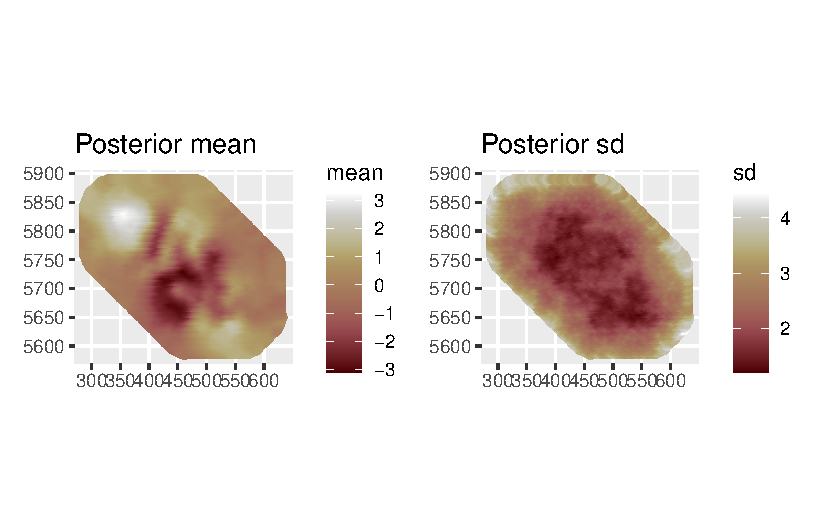
\includegraphics[keepaspectratio]{practical2_compiler_files/figure-pdf/unnamed-chunk-50-1.pdf}}
\end{center}

\textbf{Note} The posterior sd is lowest at the observation points. Note
how the posterior sd is inflated around the border, this is the ``border
effect'' due to the SPDE representation.

\subsubsection{An alternative model (including spatial
covariates)}\label{an-alternative-model-including-spatial-covariates}

We now want to check if the \texttt{depth} covariate has an influence on
the probability of presence. We do this in two different models

\begin{enumerate}
\def\labelenumi{\arabic{enumi}.}
\tightlist
\item
  \textbf{Model 1} The depth enters the model in a linear way. The
  linear predictor is then defined as:
\end{enumerate}

\[
  \eta(s) = \text{logit}(p(s)) = \beta_0 + \omega(s) + \beta_1\ \text{depth}(s)
\]

\begin{enumerate}
\def\labelenumi{\arabic{enumi}.}
\setcounter{enumi}{1}
\tightlist
\item
  \textbf{Model 1} The depth enters the model in a non linear way. The
  linear predictor is then defined as:
\end{enumerate}

\[
  \eta(s) = \text{logit}(p(s)) = \beta_0 + \omega(s) +  f(\text{depth}(s))
\] where \(f(.)\) is a smooth function. We will use a RW2 model for
this.

\begin{tcolorbox}[enhanced jigsaw, left=2mm, coltitle=black, breakable, leftrule=.75mm, colbacktitle=quarto-callout-warning-color!10!white, colframe=quarto-callout-warning-color-frame, rightrule=.15mm, colback=white, bottomtitle=1mm, opacitybacktitle=0.6, toptitle=1mm, titlerule=0mm, title={Task}, arc=.35mm, opacityback=0, bottomrule=.15mm, toprule=.15mm]

Fit model 1. Define components, observation model and use the
\texttt{bru()} function to estimate the parameters.

\textbf{Note} Use the scaled version of the covariate stored in
\texttt{depth\_r\$depth\_scaled}.

What is the liner effect of depth on the logit probability?

Take hint

The \texttt{pcod\_sf} object already contains the \texttt{depth\_scaled}
containing the squared depth values at each location. However,
\texttt{inlabru} also allows to specify a raster object directly in the
model components. If your raster contains multiple layers, then de
desired layer can be called using the \texttt{\$} symbol (e.g.,
\texttt{my\_raster\$layer\_1}).

Click here to see the solution

\begin{Shaded}
\begin{Highlighting}[]
\NormalTok{cmp }\OtherTok{=} \ErrorTok{\textasciitilde{}} \FunctionTok{Intercept}\NormalTok{(}\DecValTok{1}\NormalTok{) }\SpecialCharTok{+} \FunctionTok{space}\NormalTok{(geometry, }\AttributeTok{model =}\NormalTok{ spde\_model3) }\SpecialCharTok{+}
        \FunctionTok{covariate}\NormalTok{(depth\_r}\SpecialCharTok{$}\NormalTok{depth\_scaled, }\AttributeTok{model =} \StringTok{"linear"}\NormalTok{)}

\NormalTok{formula }\OtherTok{=}\NormalTok{ present }\SpecialCharTok{\textasciitilde{}}\NormalTok{ Intercept  }\SpecialCharTok{+}\NormalTok{ space }\SpecialCharTok{+}\NormalTok{ covariate}

\NormalTok{lik }\OtherTok{=} \FunctionTok{bru\_obs}\NormalTok{(}\AttributeTok{formula =}\NormalTok{ formula, }
              \AttributeTok{data =}\NormalTok{ pcod\_sf, }
              \AttributeTok{family =} \StringTok{"binomial"}\NormalTok{)}


\NormalTok{fit2 }\OtherTok{=} \FunctionTok{bru}\NormalTok{(cmp, lik)}
\end{Highlighting}
\end{Shaded}

\end{tcolorbox}

We now want to fit \textbf{Model 2} where we allow the effect of depth
to be non-linear. To use the RW2 model we need to \emph{group} the
values of depth into distinct classes. To do this we use the function
\texttt{inla.group()} which, by default, creates 20 groups. The we can
fit the model as usual

\begin{Shaded}
\begin{Highlighting}[]
\CommentTok{\# create the grouped variable}
\NormalTok{depth\_r}\SpecialCharTok{$}\NormalTok{depth\_group }\OtherTok{=} \FunctionTok{inla.group}\NormalTok{(}\FunctionTok{values}\NormalTok{(depth\_r}\SpecialCharTok{$}\NormalTok{depth\_scaled))}

\CommentTok{\# run the model}
\NormalTok{cmp }\OtherTok{=} \ErrorTok{\textasciitilde{}} \FunctionTok{Intercept}\NormalTok{(}\DecValTok{1}\NormalTok{) }\SpecialCharTok{+} \FunctionTok{space}\NormalTok{(geometry, }\AttributeTok{model =}\NormalTok{ spde\_model3) }\SpecialCharTok{+}
        \FunctionTok{covariate}\NormalTok{(depth\_r}\SpecialCharTok{$}\NormalTok{depth\_group, }\AttributeTok{model =} \StringTok{"rw2"}\NormalTok{)}

\NormalTok{formula }\OtherTok{=}\NormalTok{ present }\SpecialCharTok{\textasciitilde{}}\NormalTok{ Intercept  }\SpecialCharTok{+}\NormalTok{ space }\SpecialCharTok{+}\NormalTok{ covariate}

\NormalTok{lik }\OtherTok{=} \FunctionTok{bru\_obs}\NormalTok{(}\AttributeTok{formula =}\NormalTok{ formula, }
              \AttributeTok{data =}\NormalTok{ pcod\_sf, }
              \AttributeTok{family =} \StringTok{"binomial"}\NormalTok{)}


\NormalTok{fit3 }\OtherTok{=} \FunctionTok{bru}\NormalTok{(cmp, lik)}

\CommentTok{\# plot the estimated effect of depth}

\NormalTok{fit3}\SpecialCharTok{$}\NormalTok{summary.random}\SpecialCharTok{$}\NormalTok{covariate }\SpecialCharTok{\%\textgreater{}\%} 
  \FunctionTok{ggplot}\NormalTok{() }\SpecialCharTok{+} \FunctionTok{geom\_line}\NormalTok{(}\FunctionTok{aes}\NormalTok{(ID,mean)) }\SpecialCharTok{+} 
             \FunctionTok{geom\_ribbon}\NormalTok{(}\FunctionTok{aes}\NormalTok{(ID,}
                             \AttributeTok{ymin =} \StringTok{\textasciigrave{}}\AttributeTok{0.025quant}\StringTok{\textasciigrave{}}\NormalTok{, }
                             \AttributeTok{ymax =} \StringTok{\textasciigrave{}}\AttributeTok{0.975quant}\StringTok{\textasciigrave{}}\NormalTok{),}
                         \AttributeTok{alpha =} \FloatTok{0.5}\NormalTok{)}
\end{Highlighting}
\end{Shaded}

\begin{center}
\pandocbounded{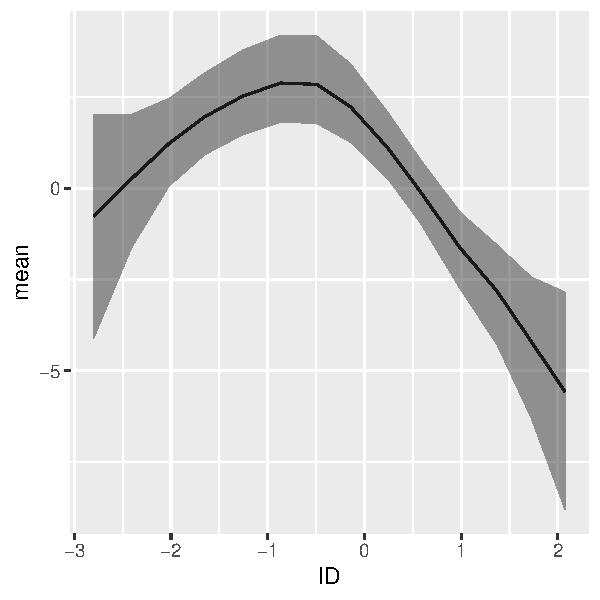
\includegraphics[keepaspectratio]{practical2_compiler_files/figure-pdf/unnamed-chunk-52-1.pdf}}
\end{center}

Instead of predicting over a grid covering the whole mesh, we can limit
our predictions to the points where the covariate is defined. We can do
this by defining a \texttt{sf} object using coordinates in the object
\texttt{depth\_r}.

\begin{Shaded}
\begin{Highlighting}[]
\NormalTok{pxl1 }\OtherTok{=} \FunctionTok{data.frame}\NormalTok{(}\FunctionTok{crds}\NormalTok{(depth\_r), }
                  \FunctionTok{as.data.frame}\NormalTok{(depth\_r}\SpecialCharTok{$}\NormalTok{depth)) }\SpecialCharTok{\%\textgreater{}\%} 
       \FunctionTok{filter}\NormalTok{(}\SpecialCharTok{!}\FunctionTok{is.na}\NormalTok{(depth)) }\SpecialCharTok{\%\textgreater{}\%}
\FunctionTok{st\_as\_sf}\NormalTok{(}\AttributeTok{coords =} \FunctionTok{c}\NormalTok{(}\StringTok{"x"}\NormalTok{,}\StringTok{"y"}\NormalTok{)) }\SpecialCharTok{\%\textgreater{}\%}\NormalTok{ dplyr}\SpecialCharTok{::}\FunctionTok{select}\NormalTok{(}\SpecialCharTok{{-}}\NormalTok{depth)}
\end{Highlighting}
\end{Shaded}

\begin{tcolorbox}[enhanced jigsaw, left=2mm, coltitle=black, breakable, leftrule=.75mm, colbacktitle=quarto-callout-warning-color!10!white, colframe=quarto-callout-warning-color-frame, rightrule=.15mm, colback=white, bottomtitle=1mm, opacitybacktitle=0.6, toptitle=1mm, titlerule=0mm, title={Task}, arc=.35mm, opacityback=0, bottomrule=.15mm, toprule=.15mm]

Create a map of predicted \emph{probability} from Model 3 by predicting
prediction over \texttt{pxl1}. You can use a inverse logit function
defined as

\begin{Shaded}
\begin{Highlighting}[]
\NormalTok{inv\_logit }\OtherTok{=} \ControlFlowTok{function}\NormalTok{(x) (}\DecValTok{1}\SpecialCharTok{+}\FunctionTok{exp}\NormalTok{(}\SpecialCharTok{{-}}\NormalTok{x))}\SpecialCharTok{\^{}}\NormalTok{(}\SpecialCharTok{{-}}\DecValTok{1}\NormalTok{)}
\end{Highlighting}
\end{Shaded}

Take hint

The \texttt{predict()} function can take as input also functions of
elements of the components you want to consider

Click here to see the solution

\begin{Shaded}
\begin{Highlighting}[]
\NormalTok{pred3  }\OtherTok{=} \FunctionTok{predict}\NormalTok{(fit3, pxl1, }\SpecialCharTok{\textasciitilde{}}\FunctionTok{inv\_logit}\NormalTok{(Intercept }\SpecialCharTok{+}\NormalTok{ space }\SpecialCharTok{+}\NormalTok{ covariate) )}

\NormalTok{pred3 }\SpecialCharTok{\%\textgreater{}\%} \FunctionTok{ggplot}\NormalTok{() }\SpecialCharTok{+} 
      \FunctionTok{geom\_sf}\NormalTok{(}\FunctionTok{aes}\NormalTok{(}\AttributeTok{color =}\NormalTok{ mean)) }\SpecialCharTok{+}
        \FunctionTok{scale\_color\_scico}\NormalTok{(}\AttributeTok{direction =} \SpecialCharTok{{-}}\DecValTok{1}\NormalTok{) }\SpecialCharTok{+}
        \FunctionTok{ggtitle}\NormalTok{(}\StringTok{"Sample from the fitted model"}\NormalTok{)}
\end{Highlighting}
\end{Shaded}

\begin{center}
\pandocbounded{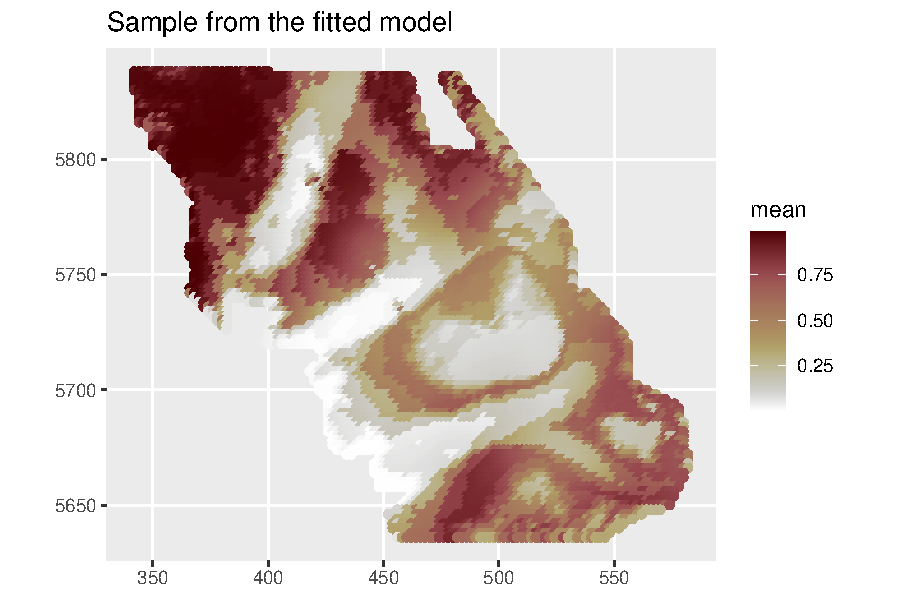
\includegraphics[keepaspectratio]{practical2_compiler_files/figure-pdf/unnamed-chunk-55-1.pdf}}
\end{center}

\end{tcolorbox}

\subsection{Point process data}\label{point-process-data}

In this practical we are going to fit a log Gaussian Cox Proces (LGCP)
model to point-referenced data. We will:

\begin{itemize}
\item
  Learn how to fit a LGCP model in \texttt{inlabru}
\item
  Learn how to add spatial covariates to the model
\item
  Learn how to do predictions
\end{itemize}

In \textbf{point processes} we measure the locations where events occur
(e.g.~trees in a forest, earthquakes) and the coordinates of such
occurrences are our data. A spatial point process is a random variable
operating in continuous space, and we observe realisations of this
variable as point patterns across space.

Consider a fixed geographical region \(A\). The set of locations at
which events occur are denoted \(\mathbf{s} = s_1,\ldots,s_n\). We let
\(N(A)\) be the random variable which represents the number of events in
region \(A\).

We typically assume that a spatial point pattern is generated by an
unique point process over the whole study area. This means that the
delimitation of the study area will affect the observed point patters.

We can define the intensity of a point process as the expected number of
events per unit area. This can also be thought of as a measure of the
density of our points. In some cases, the intensity will be constant
over space (homogeneous), while in other cases it can vary by location
(inhomogeneous or heterogenous).

In the next example we will be looking at butterflies occurrence records
obtained from the \emph{Butterflies for the New Millennium} (BNM)
monitoring scheme. The data set consists of Ringlet butterfly's
presence-only records collected by volunteers in Scotland's Cairngorms
National Park (CNP).

\subsubsection{Point-referenced data
visualization}\label{point-referenced-data-visualization}

Let's begin by loading the data which can be downloaded below:

\begin{Shaded}
\begin{Highlighting}[]
\CommentTok{\# load data files (set the correct path to where the data are stored)}
\FunctionTok{load}\NormalTok{(}\StringTok{"datasets/ringlett\_CNP.RData"}\NormalTok{)}
\NormalTok{elev\_rast }\OtherTok{=}\NormalTok{ terra}\SpecialCharTok{::}\FunctionTok{rast}\NormalTok{(}\StringTok{"datasets/elev\_CNP.tiff"}\NormalTok{)}
\end{Highlighting}
\end{Shaded}

Then, we load the geographical region of interest which can be
downloaded
\href{https://maps.gov.scot/ATOM/shapefiles/SG_CairngormsNationalPark_2010.zip}{here}
(i.e., CNP boundaries). We can use thre \texttt{st\_read} function from
the \texttt{sf} library to load the \texttt{.shp} file by specifying the
directory where you downloaded the files. For example,

\begin{Shaded}
\begin{Highlighting}[]
\NormalTok{shp\_SGC }\OtherTok{\textless{}{-}}  \FunctionTok{st\_read}\NormalTok{(}\StringTok{"datasets/SG\_CairngormsNationalPark/SG\_CairngormsNationalPark\_2010.shp"}\NormalTok{,}\AttributeTok{quiet =}\NormalTok{T)}
\end{Highlighting}
\end{Shaded}

We need to set an appropriate CRS for our shapefile:

\begin{Shaded}
\begin{Highlighting}[]
\NormalTok{shp\_SGC }\OtherTok{\textless{}{-}}\NormalTok{ shp\_SGC }\SpecialCharTok{\%\textgreater{}\%} \FunctionTok{st\_transform}\NormalTok{(}\AttributeTok{crs =} \DecValTok{27700}\NormalTok{)}
\NormalTok{shp\_SGC }\OtherTok{\textless{}{-}} \FunctionTok{st\_transform}\NormalTok{(shp\_SGC,}\FunctionTok{gsub}\NormalTok{(}\StringTok{"units=m"}\NormalTok{,}\StringTok{"units=km"}\NormalTok{,}\FunctionTok{st\_crs}\NormalTok{(shp\_SGC)}\SpecialCharTok{$}\NormalTok{proj4string)) }
\end{Highlighting}
\end{Shaded}

We can then visually verify the projections by plotting the observation
records against the spatial domain of interest as follows:

\begin{Shaded}
\begin{Highlighting}[]
\FunctionTok{ggplot}\NormalTok{()}\SpecialCharTok{+}
  \FunctionTok{geom\_sf}\NormalTok{(}\AttributeTok{data=}\NormalTok{shp\_SGC)}\SpecialCharTok{+}
  \FunctionTok{geom\_sf}\NormalTok{(}\AttributeTok{data=}\NormalTok{ringlett\_CNP,}\AttributeTok{size=}\DecValTok{2}\NormalTok{)}
\end{Highlighting}
\end{Shaded}

\begin{center}
\pandocbounded{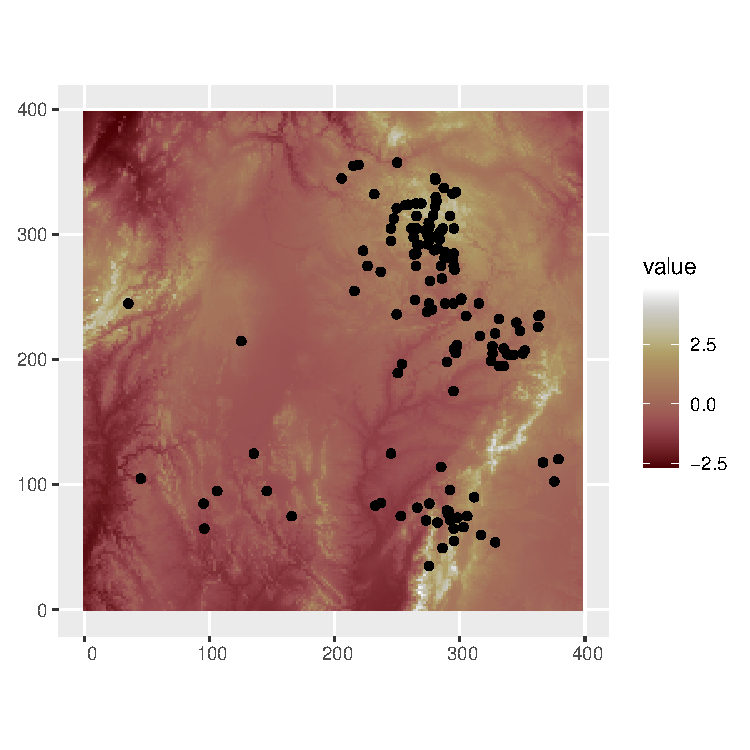
\includegraphics[keepaspectratio]{practical2_compiler_files/figure-pdf/unnamed-chunk-82-1.pdf}}
\end{center}

\begin{tcolorbox}[enhanced jigsaw, left=2mm, coltitle=black, breakable, leftrule=.75mm, colbacktitle=quarto-callout-warning-color!10!white, colframe=quarto-callout-warning-color-frame, rightrule=.15mm, colback=white, bottomtitle=1mm, opacitybacktitle=0.6, toptitle=1mm, titlerule=0mm, title={Task}, arc=.35mm, opacityback=0, bottomrule=.15mm, toprule=.15mm]

Using \texttt{tidyterra} and \texttt{ggplot}, produce a map of the
elevation profile in the CNP and overlay the spatial point pattern of
the Ringlet butterfly occurrence records. Use an appropriate colouring
scheme for the elevation values. Do you see any pattern?

Take hint

You can use the \texttt{geom\_spatraster()} to add a raster layer to a
ggplot object. Furthermore the \texttt{scico} library contains a nice
range of coloring palettes you can choose, type
\texttt{scico\_palette\_show()} to see the color palettes that are
available.

Click here to see the solution

\begin{Shaded}
\begin{Highlighting}[]
\FunctionTok{library}\NormalTok{(ggplot2)}
\FunctionTok{library}\NormalTok{(tidyterra)}
\FunctionTok{library}\NormalTok{(scico)}

\FunctionTok{ggplot}\NormalTok{()}\SpecialCharTok{+} 
\NormalTok{  tidyterra}\SpecialCharTok{::}\FunctionTok{geom\_spatraster}\NormalTok{(}\AttributeTok{data=}\NormalTok{elev\_rast)}\SpecialCharTok{+}
  \FunctionTok{geom\_sf}\NormalTok{(}\AttributeTok{data=}\NormalTok{ringlett\_CNP,}\AttributeTok{color=}\StringTok{"white"}\NormalTok{,}\AttributeTok{size=}\DecValTok{2}\NormalTok{)}\SpecialCharTok{+}
  \FunctionTok{geom\_sf}\NormalTok{(}\AttributeTok{data=}\NormalTok{ringlett\_CNP,}\AttributeTok{color=}\StringTok{"forestgreen"}\NormalTok{,}\AttributeTok{size=}\DecValTok{1}\NormalTok{)}\SpecialCharTok{+}
  \FunctionTok{scale\_fill\_scico}\NormalTok{(}\AttributeTok{name =} \StringTok{"Elevation (m.a.s.l)"}\NormalTok{,}
                   \AttributeTok{palette =} \StringTok{"devon"}\NormalTok{,}
                   \AttributeTok{na.value =} \StringTok{"transparent"}\NormalTok{ )}
\end{Highlighting}
\end{Shaded}

\begin{center}
\pandocbounded{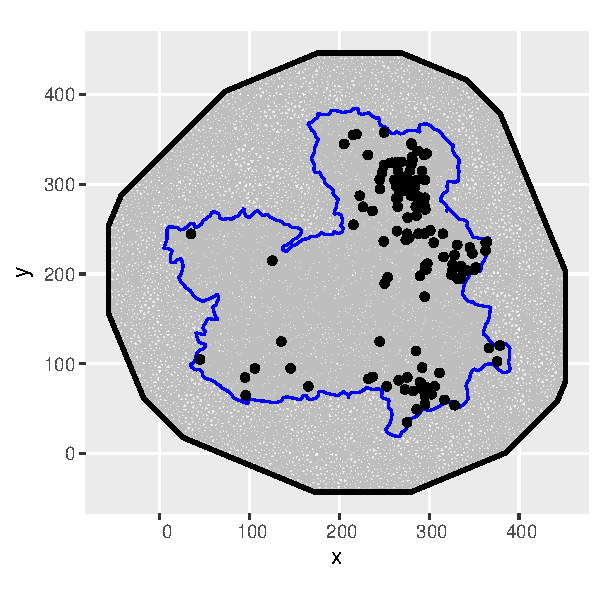
\includegraphics[keepaspectratio]{practical2_compiler_files/figure-pdf/unnamed-chunk-83-1.pdf}}
\end{center}

\end{tcolorbox}

\subsubsection{Workflow for Fitting a LGCP
model}\label{workflow-for-fitting-a-lgcp-model}

The procedure for fitting a point process model in \texttt{inlabru},
specifically a log-Gaussian Cox process, follows a similar workflow to
that of a geostatistical model, these are:

\begin{enumerate}
\def\labelenumi{\arabic{enumi}.}
\tightlist
\item
  Build the mesh
\item
  Define the SPDE representation of the spatial GF. This includes
  defining the priors for the range and sd of the spatial GF
\item
  Define the \emph{components} of the linear predictor. This includes
  the spatial GF and all eventual covariates.
\item
  Define the observational model
\item
  Run the Model
\end{enumerate}

\paragraph{Step 1. Building the mesh for a
LGCP}\label{step-1.-building-the-mesh-for-a-lgcp}

First, we need to create the mesh used to approximate the random field.
When analyzing point patterns, mesh nodes (integration points) are not
typically placed at point locations. Instead, a mesh is created using
the \texttt{fm\_mesh\_2d()}function from the \texttt{fmesher} library
with boundary being our study area.

Key parameters in mesh construction include: \texttt{max.edge} for
maximum triangle edge lengths, \texttt{offset} for inner and outer
extensions (to prevent edge effects), and cutoff to avoid overly small
triangles in clustered areas.

\begin{tcolorbox}[enhanced jigsaw, left=2mm, coltitle=black, breakable, leftrule=.75mm, colbacktitle=quarto-callout-note-color!10!white, colframe=quarto-callout-note-color-frame, rightrule=.15mm, colback=white, bottomtitle=1mm, opacitybacktitle=0.6, toptitle=1mm, titlerule=0mm, title=\textcolor{quarto-callout-note-color}{\faInfo}\hspace{0.5em}{Note}, arc=.35mm, opacityback=0, bottomrule=.15mm, toprule=.15mm]

\textbf{General guidelines for creating the mesh}

\begin{enumerate}
\def\labelenumi{\arabic{enumi}.}
\tightlist
\item
  Create triangulation meshes with \texttt{fm\_mesh\_2d()}
\item
  Move undesired boundary effects away from the domain of interest by
  extending to a smooth external boundary
\item
  Use a coarser resolution in the extension to reduce computational cost
  (\texttt{max.edge=c(inner,\ outer)})
\item
  Use a fine resolution (subject to available computational resources)
  for the domain of interest (inner correlation range) and filter out
  small input point clusters (0 \textless{} \texttt{cutoff} \textless{}
  inner)
\item
  Coastlines and similar can be added to the domain specification in
  \texttt{fm\_mesh\_2d()} through the \texttt{boundary} argument.
\end{enumerate}

\end{tcolorbox}

\begin{Shaded}
\begin{Highlighting}[]
\CommentTok{\# mesh options}
\NormalTok{max.edge }\OtherTok{=} \DecValTok{2}
\NormalTok{bound.outer }\OtherTok{=} \DecValTok{10}

\NormalTok{mesh }\OtherTok{\textless{}{-}} \FunctionTok{fm\_mesh\_2d}\NormalTok{(}\AttributeTok{boundary =}\NormalTok{ shp\_SGC,}
                   \AttributeTok{max.edge =} \FunctionTok{c}\NormalTok{(}\DecValTok{1}\NormalTok{,}\DecValTok{3}\NormalTok{)}\SpecialCharTok{*}\NormalTok{max.edge,}
                   \AttributeTok{offset=}\FunctionTok{c}\NormalTok{(max.edge, bound.outer),}
                   \AttributeTok{cutoff =} \FloatTok{1.5}\NormalTok{,}
                   \AttributeTok{crs=}\FunctionTok{st\_crs}\NormalTok{(shp\_SGC))}

\FunctionTok{ggplot}\NormalTok{() }\SpecialCharTok{+} \FunctionTok{gg}\NormalTok{(mesh) }\SpecialCharTok{+} \FunctionTok{geom\_sf}\NormalTok{(}\AttributeTok{data=}\NormalTok{ringlett\_CNP)}
\end{Highlighting}
\end{Shaded}

\begin{center}
\pandocbounded{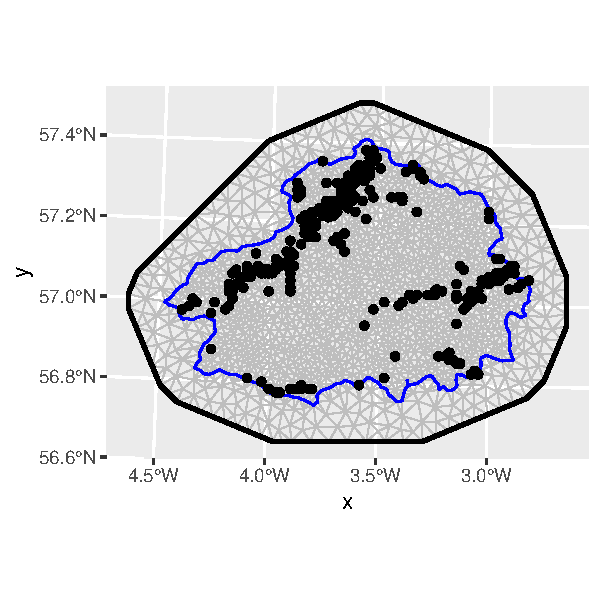
\includegraphics[keepaspectratio]{practical2_compiler_files/figure-pdf/unnamed-chunk-84-1.pdf}}
\end{center}

\paragraph{Step 2. Defining the SPDE
model}\label{step-2.-defining-the-spde-model}

We can now define our SPDE model using the \texttt{inla.spde2.pcmatern}
function. To help us chose some sensible model parameters it is often
useful to consider the spatial extension of our study.

\begin{Shaded}
\begin{Highlighting}[]
\FunctionTok{st\_area}\NormalTok{(shp\_SGC)}
\end{Highlighting}
\end{Shaded}

\begin{verbatim}
4528.099 [km^2]
\end{verbatim}

We can use PC-priors for the range \(\rho\) and the standard deviation
\(\sigma\) of the Matérn process

\begin{itemize}
\item
  Define the prior for the range
  \texttt{prior.range\ \ =\ (range0,Prange)}
  \(\text{Prob}(\rho<\rho_0) = p_{\rho}\)
\item
  Define the prior for the range
  \texttt{prior.sigma\ \ =\ (sigma0,Psigma)}
  \(\text{Prob}(\sigma>\sigma_0) = p_{\sigma}\)
\end{itemize}

\begin{Shaded}
\begin{Highlighting}[]
\NormalTok{matern }\OtherTok{\textless{}{-}} \FunctionTok{inla.spde2.pcmatern}\NormalTok{(mesh,}
                              \AttributeTok{prior.range =} \FunctionTok{c}\NormalTok{(}\DecValTok{20}\NormalTok{, }\FloatTok{0.5}\NormalTok{), }\CommentTok{\# P(range \textless{} 20) = 0.5}
                              \AttributeTok{prior.sigma =} \FunctionTok{c}\NormalTok{(}\DecValTok{1}\NormalTok{, }\FloatTok{0.5}\NormalTok{))  }\CommentTok{\# P(sigma \textgreater{} 1) = 0.5}
\end{Highlighting}
\end{Shaded}

Now, for a point process models, the spatial covariates (i.e., the
elevation raster) has to be also projected outside the outer mesh for
computational purposes. We can achieve this using the following code:

\begin{Shaded}
\begin{Highlighting}[]
\FunctionTok{library}\NormalTok{(stars)}

\CommentTok{\# Standardize the raster }
\NormalTok{elev\_rast }\OtherTok{\textless{}{-}} \FunctionTok{scale}\NormalTok{(elev\_rast)}
\CommentTok{\# Extend raster ext by a factor of 1.5}
\NormalTok{re }\OtherTok{\textless{}{-}} \FunctionTok{extend}\NormalTok{(elev\_rast, }\FunctionTok{ext}\NormalTok{(elev\_rast)}\SpecialCharTok{*}\FloatTok{1.5}\NormalTok{)}
\CommentTok{\# Convert to spatial object}
\NormalTok{re\_df }\OtherTok{\textless{}{-}}\NormalTok{ re }\SpecialCharTok{\%\textgreater{}\%}\NormalTok{ stars}\SpecialCharTok{::}\FunctionTok{st\_as\_stars}\NormalTok{() }\SpecialCharTok{\%\textgreater{}\%}  \FunctionTok{st\_as\_sf}\NormalTok{(}\AttributeTok{na.rm=}\NormalTok{F)}
\CommentTok{\# fill in missing values using the original raster }
\NormalTok{re\_df}\SpecialCharTok{$}\NormalTok{GBR\_elv\_msk }\OtherTok{\textless{}{-}} \FunctionTok{bru\_fill\_missing}\NormalTok{(elev\_rast,re\_df,re\_df}\SpecialCharTok{$}\NormalTok{GBR\_elv\_msk)}
\CommentTok{\# rasterize}
\NormalTok{elev\_rast\_p }\OtherTok{\textless{}{-}}\NormalTok{ stars}\SpecialCharTok{::}\FunctionTok{st\_rasterize}\NormalTok{(re\_df) }\SpecialCharTok{\%\textgreater{}\%} \FunctionTok{rast}\NormalTok{()}
\CommentTok{\# visualize}
\FunctionTok{plot}\NormalTok{(elev\_rast\_p)}
\end{Highlighting}
\end{Shaded}

\begin{center}
\pandocbounded{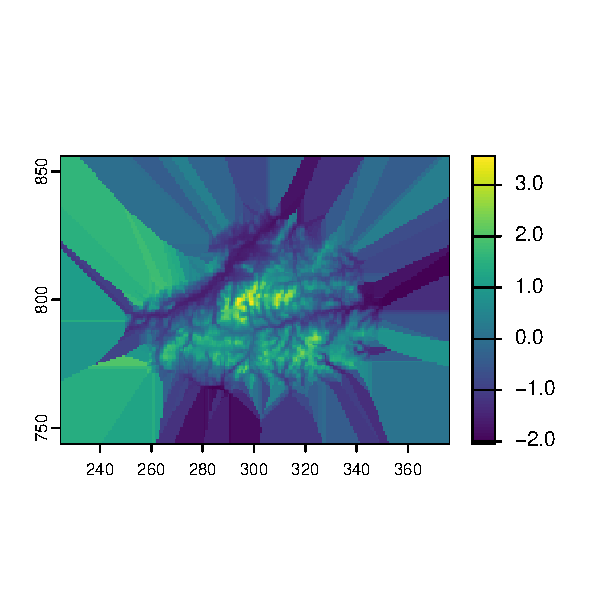
\includegraphics[keepaspectratio]{practical2_compiler_files/figure-pdf/unnamed-chunk-87-1.pdf}}
\end{center}

\paragraph{Step 3. Defining model
components}\label{step-3.-defining-model-components}

\textbf{Stage 1} Model for the response

The total number of points in the study region is a Poisson random
variable with a spatially varying intensity and log-likelihood given by
:

\[
l(\beta;s) = \sum_{i=1}^m \log [\lambda(s_i)] - \int_A \lambda(s)ds.
\]

The integral in this expression can be interpreted as the expected
number of points in the whole study region. However, the integral of the
intensity function has no close form solution and thus we need to
approximate it using numerical integration. Luckuly, LGCPs are latent
Gaussian models and they may be fitted using INLA.

\textbf{Stage 2} Latent field model

We will model the Ringlet distribution as a point process whose
intensity function \(\lambda(s)\) is additive on the log-scale:

\[
\eta(s) = \log (\lambda(s))= \beta_0 +  \mathbf{x}'(s)\beta + \omega(s),
\]

Here, \(\mathbf{x}(s)\) is a set of covariates detected at location
\(s\) with linear fixed effects \(\beta\) to be estimated, and
\(\omega(s)\) is the Matérn Gaussian field capturing the spatial
structure of all the locations where species have been observed (The
location where a species occur are assumed to be independent given the
Gaussian field).

In this exercise, we will use elevation as our covariate as it seems to
be closely related to the distribution of the Ringlet butterfly.

\textbf{Stage 3} Hyperparameters

The hyperparameters of the model are \(\rho\) and \(\sigma\)
corresponding to

\[
\omega(s)\sim \text{  GF with range } \rho\  \text{ and maginal variance }\ \sigma^2
\]

\textbf{NOTE} In this case the linear predictor \(\eta(s)\) consists of
three components.

After the mesh and a SPDE representation of the spatial GF have been
defined, the model components can be specified using the formula syntax
(recall that this allows users to choose meaningful names for model
components).

\begin{Shaded}
\begin{Highlighting}[]
\NormalTok{cmp\_lgcp }\OtherTok{\textless{}{-}}\NormalTok{  geometry }\SpecialCharTok{\textasciitilde{}}  \FunctionTok{Intercept}\NormalTok{(}\DecValTok{1}\NormalTok{)  }\SpecialCharTok{+} 
  \FunctionTok{elevation}\NormalTok{(elev\_rast\_p, }\AttributeTok{model =} \StringTok{"linear"}\NormalTok{) }\SpecialCharTok{+}
  \FunctionTok{grf}\NormalTok{(geometry, }\AttributeTok{model =}\NormalTok{ matern)}
\end{Highlighting}
\end{Shaded}

Here the labels \texttt{Intercept}, \texttt{elevation} (elevation
effect) and \texttt{grf} (an abbreviation of Gaussian random field) are
used to name the components of the model but they equally well could be
something else.

Now, notice that we have called the \texttt{elev\_rast\_p} raster data
within the \texttt{elevation} component. Recall that
\texttt{inlabru}provides support for \texttt{sf} and \texttt{terra} data
structures, allowing it to extract information from spatial data
objects. This is particularly relevant for LGCP, as spatial covariates
(e.g., the elevation raster) must be available across the whole study
area (including the outer mesh).

\begin{Shaded}
\begin{Highlighting}[]
\NormalTok{formula }\OtherTok{=}\NormalTok{ geometry }\SpecialCharTok{\textasciitilde{}}\NormalTok{ Intercept  }\SpecialCharTok{+}\NormalTok{ elevation }\SpecialCharTok{+}\NormalTok{ grf}
\end{Highlighting}
\end{Shaded}

Recall that in an \texttt{sf} object, the geo-referenced information of
our points is stored in the \texttt{geometry} column, and hence we
specify this as our response

\paragraph{Step 4. Defining th observational
model}\label{step-4.-defining-th-observational-model}

\texttt{inlabru} has support for latent Gaussian Cox processes through
the \texttt{cp} likelihood family:

\begin{Shaded}
\begin{Highlighting}[]
\NormalTok{lik }\OtherTok{=} \FunctionTok{bru\_obs}\NormalTok{(}\AttributeTok{formula =}\NormalTok{ formula, }
              \AttributeTok{data =}\NormalTok{ ringlett\_CNP, }
              \AttributeTok{family =} \StringTok{"cp"}\NormalTok{,}
              \AttributeTok{samplers =}\NormalTok{ shp\_SGC,}
              \AttributeTok{domain =} \FunctionTok{list}\NormalTok{(}\AttributeTok{geometry =}\NormalTok{ mesh))}
\end{Highlighting}
\end{Shaded}

Notice that we have supplied an \texttt{sf} object as our data. LGCPs
can be fitted using an \texttt{sf} points object to describe the
locations of the observed points and an \texttt{sf} polygon object to
define the observation window (\texttt{samplers} in the code above).

\subsubsection{Step 5. Run the model}\label{step-5.-run-the-model-1}

Finally, we can fit the model as usual

\begin{Shaded}
\begin{Highlighting}[]
\NormalTok{fit\_lgcp }\OtherTok{=} \FunctionTok{bru}\NormalTok{(cmp\_lgcp,lik)}
\end{Highlighting}
\end{Shaded}

Posterior summaries of fixed effects and hyper parameters can be
obtained using the \texttt{summary()} function.

\begin{Shaded}
\begin{Highlighting}[]
\FunctionTok{summary}\NormalTok{(fit\_lgcp)}
\end{Highlighting}
\end{Shaded}

\begin{table}
\fontsize{12.0pt}{14.0pt}\selectfont
\begin{tabular*}{\linewidth}{@{\extracolsep{\fill}}rrrrrr}
\toprule
mean & sd & 0.025quant & 0.5quant & 0.975quant & mode \\ 
\midrule\addlinespace[2.5pt]
-4.72 & 0.31 & -5.37 & -4.71 & -4.14 & -4.71 \\ 
-2.21 & 0.16 & -2.52 & -2.21 & -1.90 & -2.21 \\ 
22.12 & 10.69 & 8.76 & 19.75 & 49.63 & 15.86 \\ 
0.48 & 0.13 & 0.27 & 0.47 & 0.76 & 0.45 \\ 
\bottomrule
\end{tabular*}
\end{table}

\subsubsection{Model predictions}\label{model-predictions}

Model predictions can be computed using the \texttt{predict} function by
supplying the coordinates where the covariate is defined. We can do this
by defining a \texttt{sf} object using coordinates in our original
raster data.

\begin{Shaded}
\begin{Highlighting}[]
\NormalTok{pxl1 }\OtherTok{=} \FunctionTok{data.frame}\NormalTok{(}\FunctionTok{crds}\NormalTok{(elev\_rast), }
                  \FunctionTok{as.data.frame}\NormalTok{(elev\_rast}\SpecialCharTok{$}\NormalTok{GBR\_elv\_msk)) }\SpecialCharTok{\%\textgreater{}\%} 
       \FunctionTok{filter}\NormalTok{(}\SpecialCharTok{!}\FunctionTok{is.na}\NormalTok{(GBR\_elv\_msk)) }\SpecialCharTok{\%\textgreater{}\%}
\FunctionTok{st\_as\_sf}\NormalTok{(}\AttributeTok{coords =} \FunctionTok{c}\NormalTok{(}\StringTok{"x"}\NormalTok{,}\StringTok{"y"}\NormalTok{)) }\SpecialCharTok{\%\textgreater{}\%}
\NormalTok{  dplyr}\SpecialCharTok{::}\FunctionTok{select}\NormalTok{(}\SpecialCharTok{{-}}\NormalTok{GBR\_elv\_msk)}
\end{Highlighting}
\end{Shaded}

The formula object for the prediction can be a generic R expression that
references model components using the user-defined names.

The \texttt{predict()} method returns an object in the same data format
as was used in the predict call which, in this case, is an \texttt{sf}
points object.

Support for plotting \texttt{sf} data objects is available in the
\texttt{ggplot2} package.

\section{Model predictions}

\pandocbounded{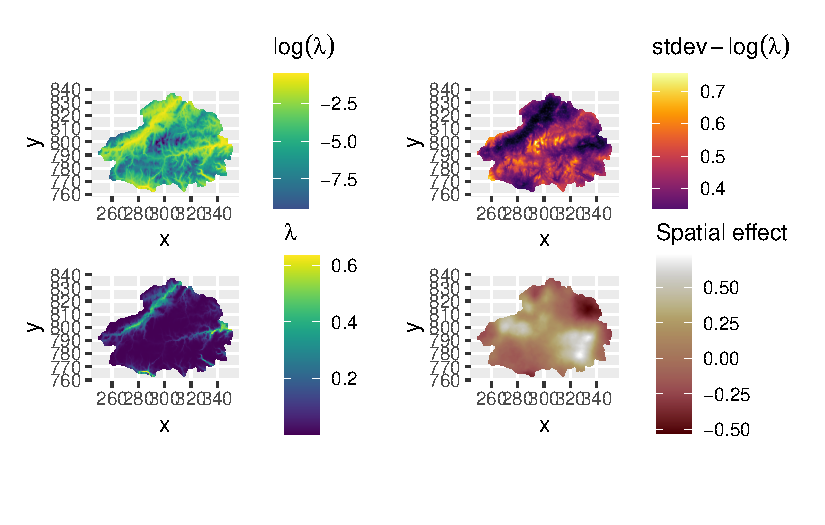
\includegraphics[keepaspectratio]{practical2_compiler_files/figure-pdf/unnamed-chunk-95-1.pdf}}

\section{R Code}

\begin{Shaded}
\begin{Highlighting}[]
\NormalTok{lgcp\_pred }\OtherTok{\textless{}{-}} \FunctionTok{predict}\NormalTok{(}
\NormalTok{  fit\_lgcp,}
\NormalTok{  pxl1,}
  \SpecialCharTok{\textasciitilde{}} \FunctionTok{data.frame}\NormalTok{(}
    \AttributeTok{lambda =} \FunctionTok{exp}\NormalTok{(Intercept }\SpecialCharTok{+}\NormalTok{ elevation }\SpecialCharTok{+}\NormalTok{ grf), }\CommentTok{\# intensity}
    \AttributeTok{loglambda =}\NormalTok{ Intercept }\SpecialCharTok{+}\NormalTok{ elevation }\SpecialCharTok{+}\NormalTok{grf,  }\CommentTok{\#log{-}intensity}
    \AttributeTok{GF =}\NormalTok{ grf }\CommentTok{\# matern field}
\NormalTok{  )}
\NormalTok{)}

\CommentTok{\# predicted log intensity}
\FunctionTok{ggplot}\NormalTok{() }\SpecialCharTok{+} \FunctionTok{gg}\NormalTok{(lgcp\_pred}\SpecialCharTok{$}\NormalTok{loglambda, }\AttributeTok{geom =} \StringTok{"tile"}\NormalTok{) }
\CommentTok{\# standard deviation of the predicted log intensity}
\FunctionTok{ggplot}\NormalTok{() }\SpecialCharTok{+} \FunctionTok{gg}\NormalTok{(lgcp\_pred}\SpecialCharTok{$}\NormalTok{loglambda, }\AttributeTok{geom =} \StringTok{"tile"}\NormalTok{,}\FunctionTok{aes}\NormalTok{(}\AttributeTok{fill=}\NormalTok{sd)) }
\CommentTok{\# predicted intensity}
\FunctionTok{ggplot}\NormalTok{() }\SpecialCharTok{+}  \FunctionTok{gg}\NormalTok{(lgcp\_pred}\SpecialCharTok{$}\NormalTok{lambda, }\AttributeTok{geom =} \StringTok{"tile"}\NormalTok{) }
\CommentTok{\# spatial field}
\FunctionTok{ggplot}\NormalTok{() }\SpecialCharTok{+}  \FunctionTok{gg}\NormalTok{(lgcp\_pred}\SpecialCharTok{$}\NormalTok{GF, }\AttributeTok{geom =} \StringTok{"tile"}\NormalTok{) }
\end{Highlighting}
\end{Shaded}





\end{document}
